\documentclass[a4paper,12pt]{report}
\usepackage{graphicx}
\title{Tugas pemrograman 2}
\author{idam fadilah}
\date{16 oktober 2019}
\begin{document}


\maketitle

\chapter{Python}
\section{Sejarah python}
\paragraph{}
Python diciptakan oleh guido van rossum di centrum wiskunde \& informatica (CWI), Belanda pada tahun 1990-an. Asal usul nama python sendiri sebenarnya tidak ada hubungannya dengan nama ular, tetapi nama python ini berasal dari nama monty python yang merupakan grup komedi inggris kegemaran Guido. Bahasa python terinspirasi dari bahasa ABC. Python bersifat open source sehingga ribuan orang telah berkontribusi dalam mengembangkan bahasa ini. Sampai saat ini Guido masih menjadi penulis utama python.\\
tanggal rilis Python versi mayor dan minor :
\begin{itemize}
	\item Python 1.0 – 01/1994
	\item Python 1.2 – 10/04/1995
	\item Python 1.3 – 12/10/1995
	\item Python 1.4 – 25/10/1996
	\item Python 1.5 – 31/12/1997
	\item Python 1.6 – 5/09/2000
	\item Python 2.0 – 16/10/2000
	\item Python 2.1 – 17/04/2001
	\item Python 2.2 – 21/12/2001
	\item Python 2.3 – 29/07/2003
	\item Python 2.4 – 30/11/2004
	\item Python 2.5 – 19/09/2006
	\item Python 2.6 – 1/10/2008
	\item Python 2.7 – 3/07/2010
	\item Python 3.0 – 3/12/2008
	\item Python 3.1 – 27/06/2009
	\item Python 3.2 – 20/02/2011
	\item Python 3.3 – 29/09/2012
	\item Python 3.4 – 16/03/2014
	\item Python 3.5 – 13/09/2015
	\item Python 3.6 – 23/12/2016
	\item Python 3.7 – 27/06/2018
	
	
\end{itemize}
\section{Perbedaaan python 2 dan 3}

\paragraph{}
perbedaan python 2 dan 3 terdapat pada penulisan syntax dan lain-lain
Syntax untuk mencetak huruf atau yang lain :
 \begin{itemize}
 	\item python 2 : print "halo dunia"
 	\item python 3 : print("halo dunia")
 \end{itemize}
Syntax untuk meminta inputan user :
 \begin{itemize}
	\item python 2 : hero = raw\_input(‘masukkan nama hero anda : ‘)
	\item python 3 : hero = input(“masukkan nama hero anda : “)
\end{itemize}
hasil pembagian :
 \begin{itemize}
	\item python 2 : pembagian floor division (contoh : 3/2 maka hasilnya 1)
	\item python 3 : oembagian lebih inituitif (contoh : 3/2 maka hasilnya 1,5)
\end{itemize}
\chapter{Instalasi}
\graphicspath{{gambar/anaconda}}
\section{Instalasi anaconda}
\paragraph{}
\begin{itemize}
	\item Kunjungi website anaconda (https://www.anaconda.com/distribution/\#download-section), download python sesuai dengan sistem operasi yang dipakai\\
	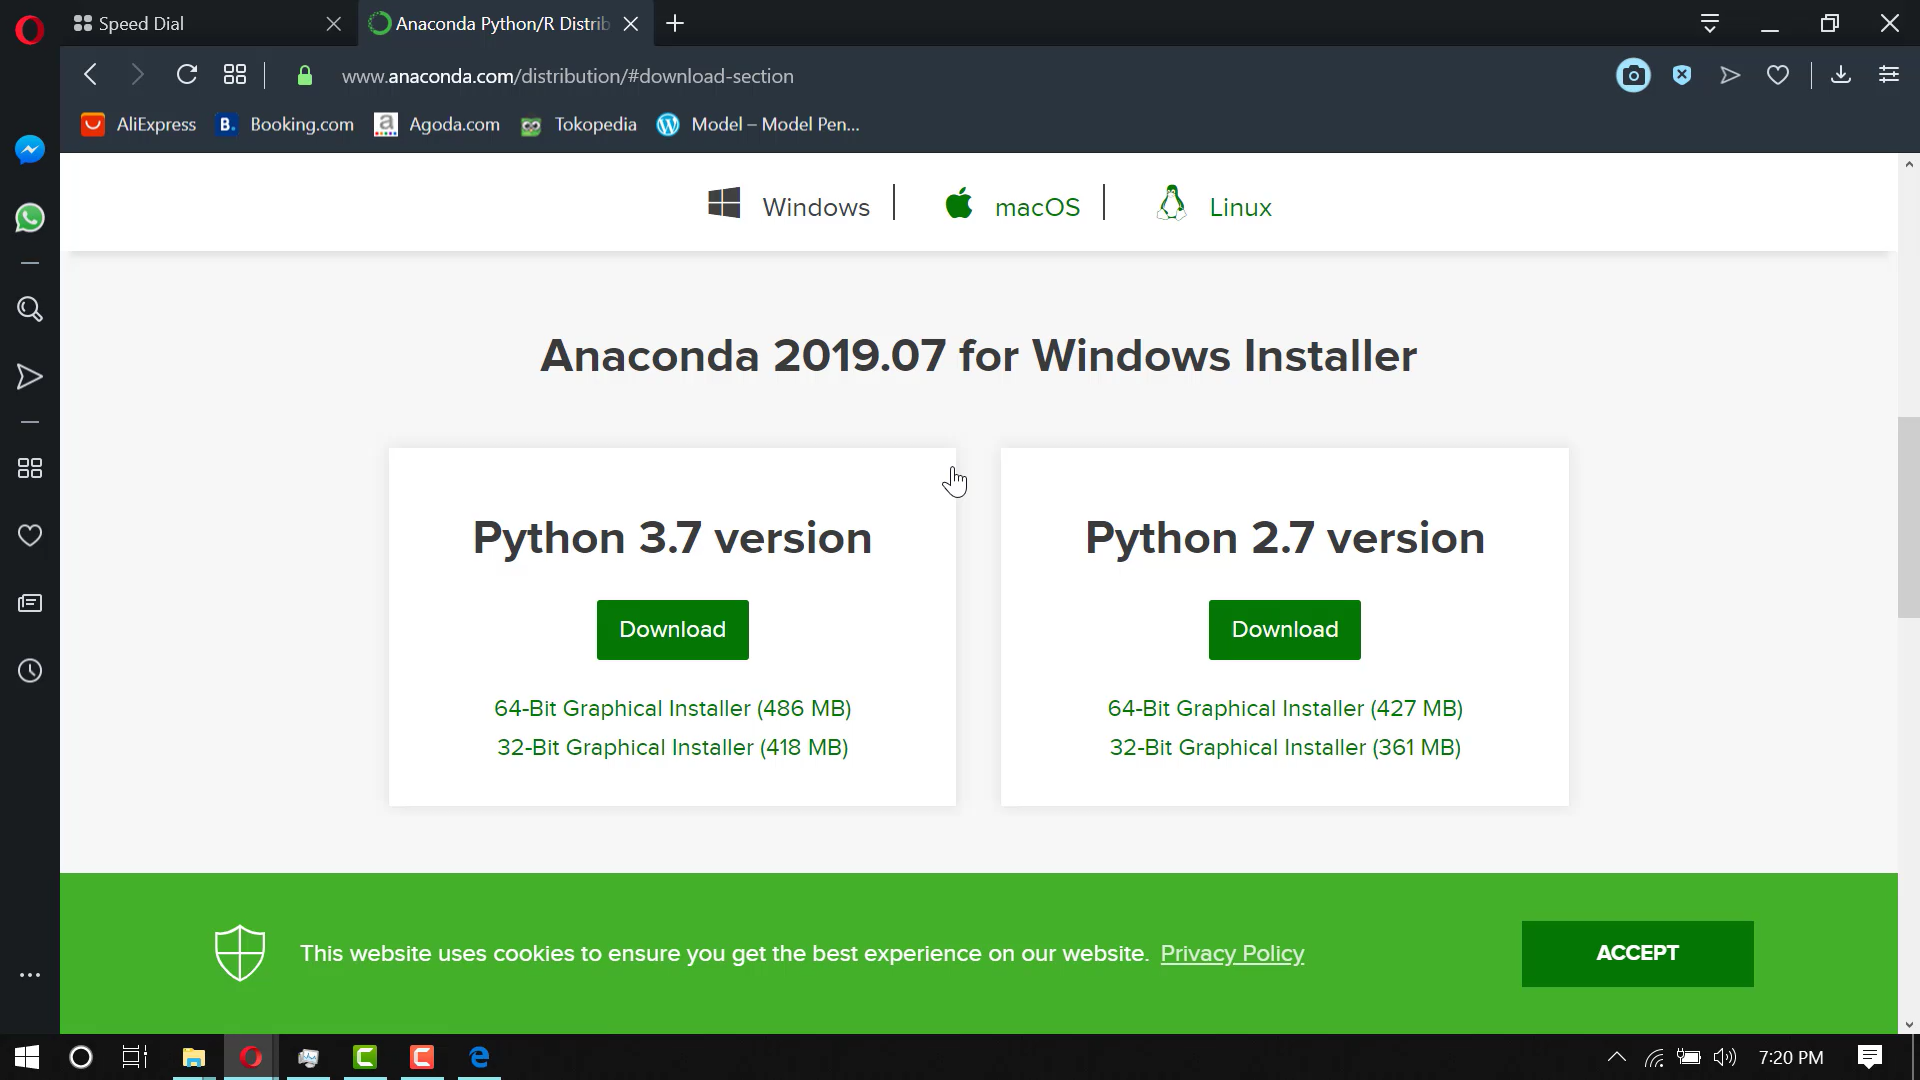
\includegraphics[width=7.5cm]{gambar/anaconda/anaconda1.png} 
	\item Buka file installer, Klik "next"\\
	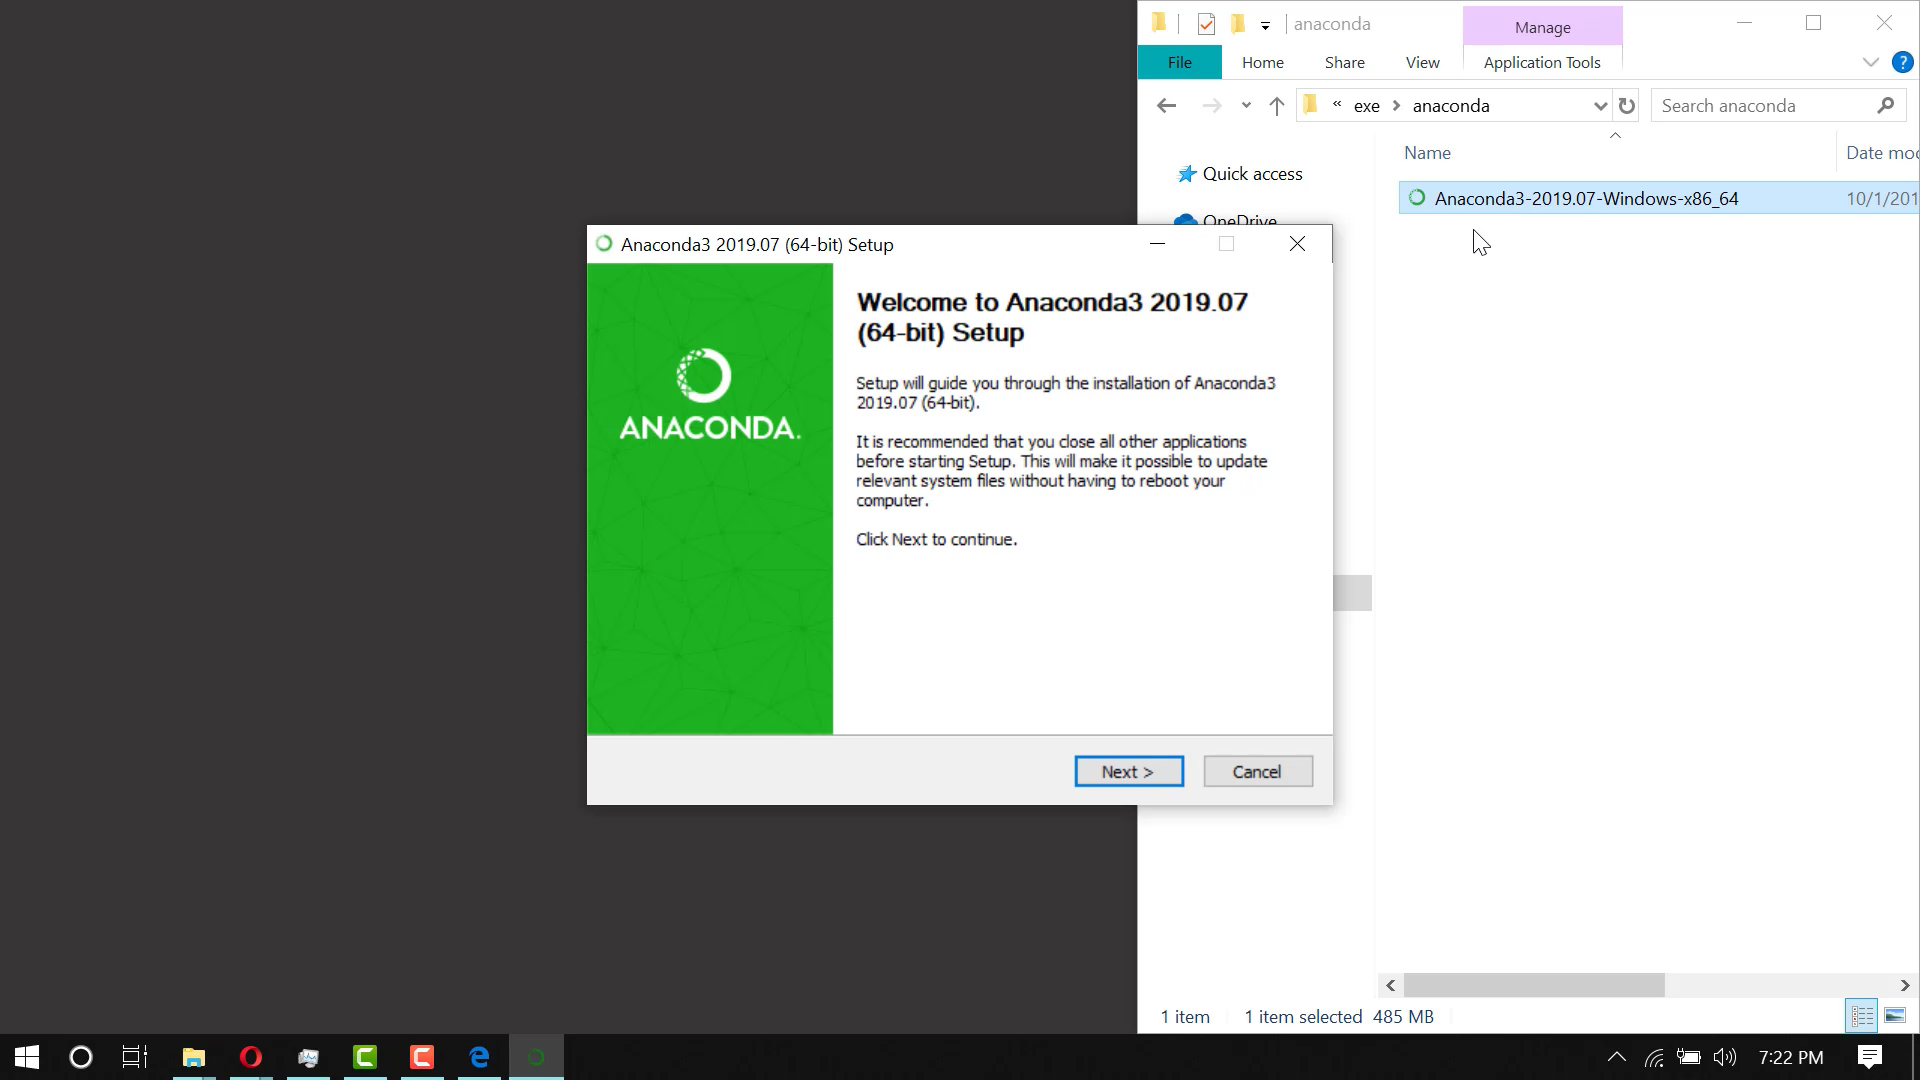
\includegraphics[width=7.5cm]{gambar/anaconda/Screenshot (60).png} 
	\item Klik "i agree"\\
	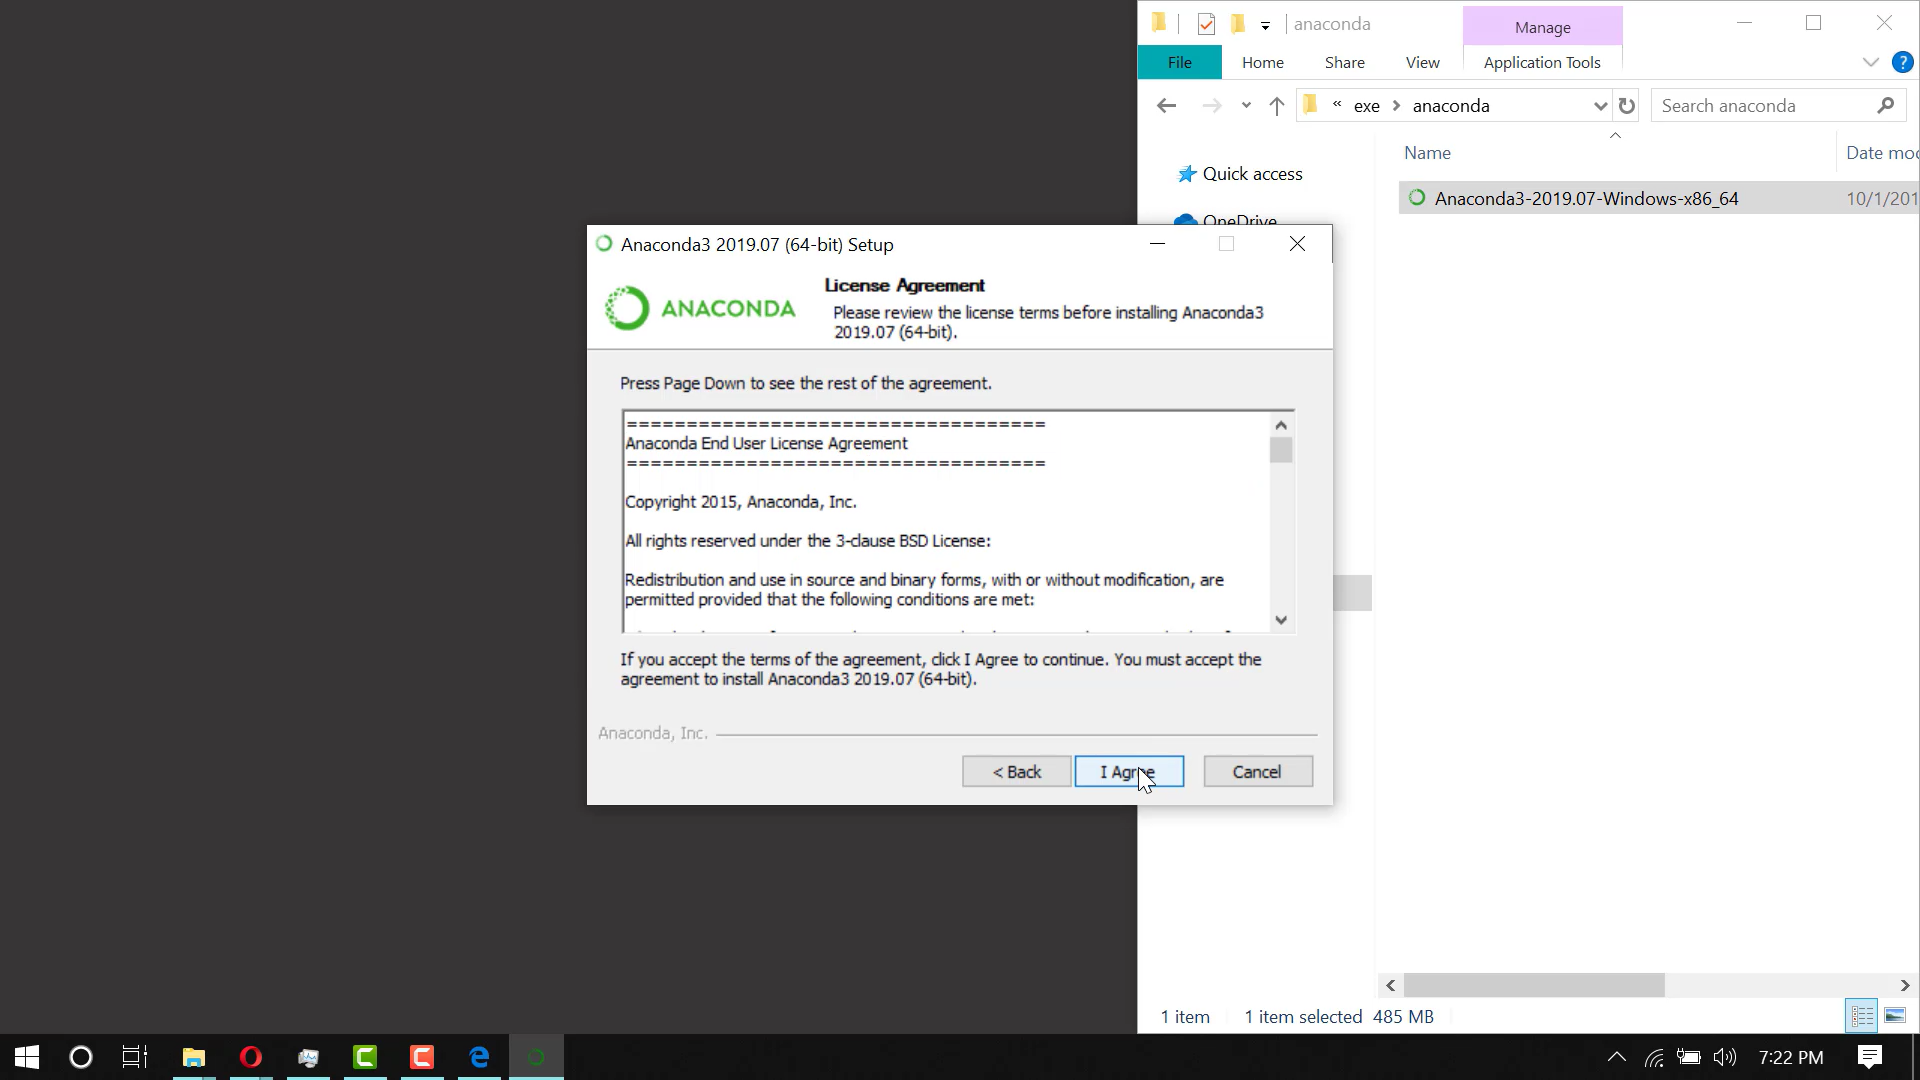
\includegraphics[width=7.5cm]{gambar/anaconda/Screenshot (61).png} 
	\item Klik "next"\\
	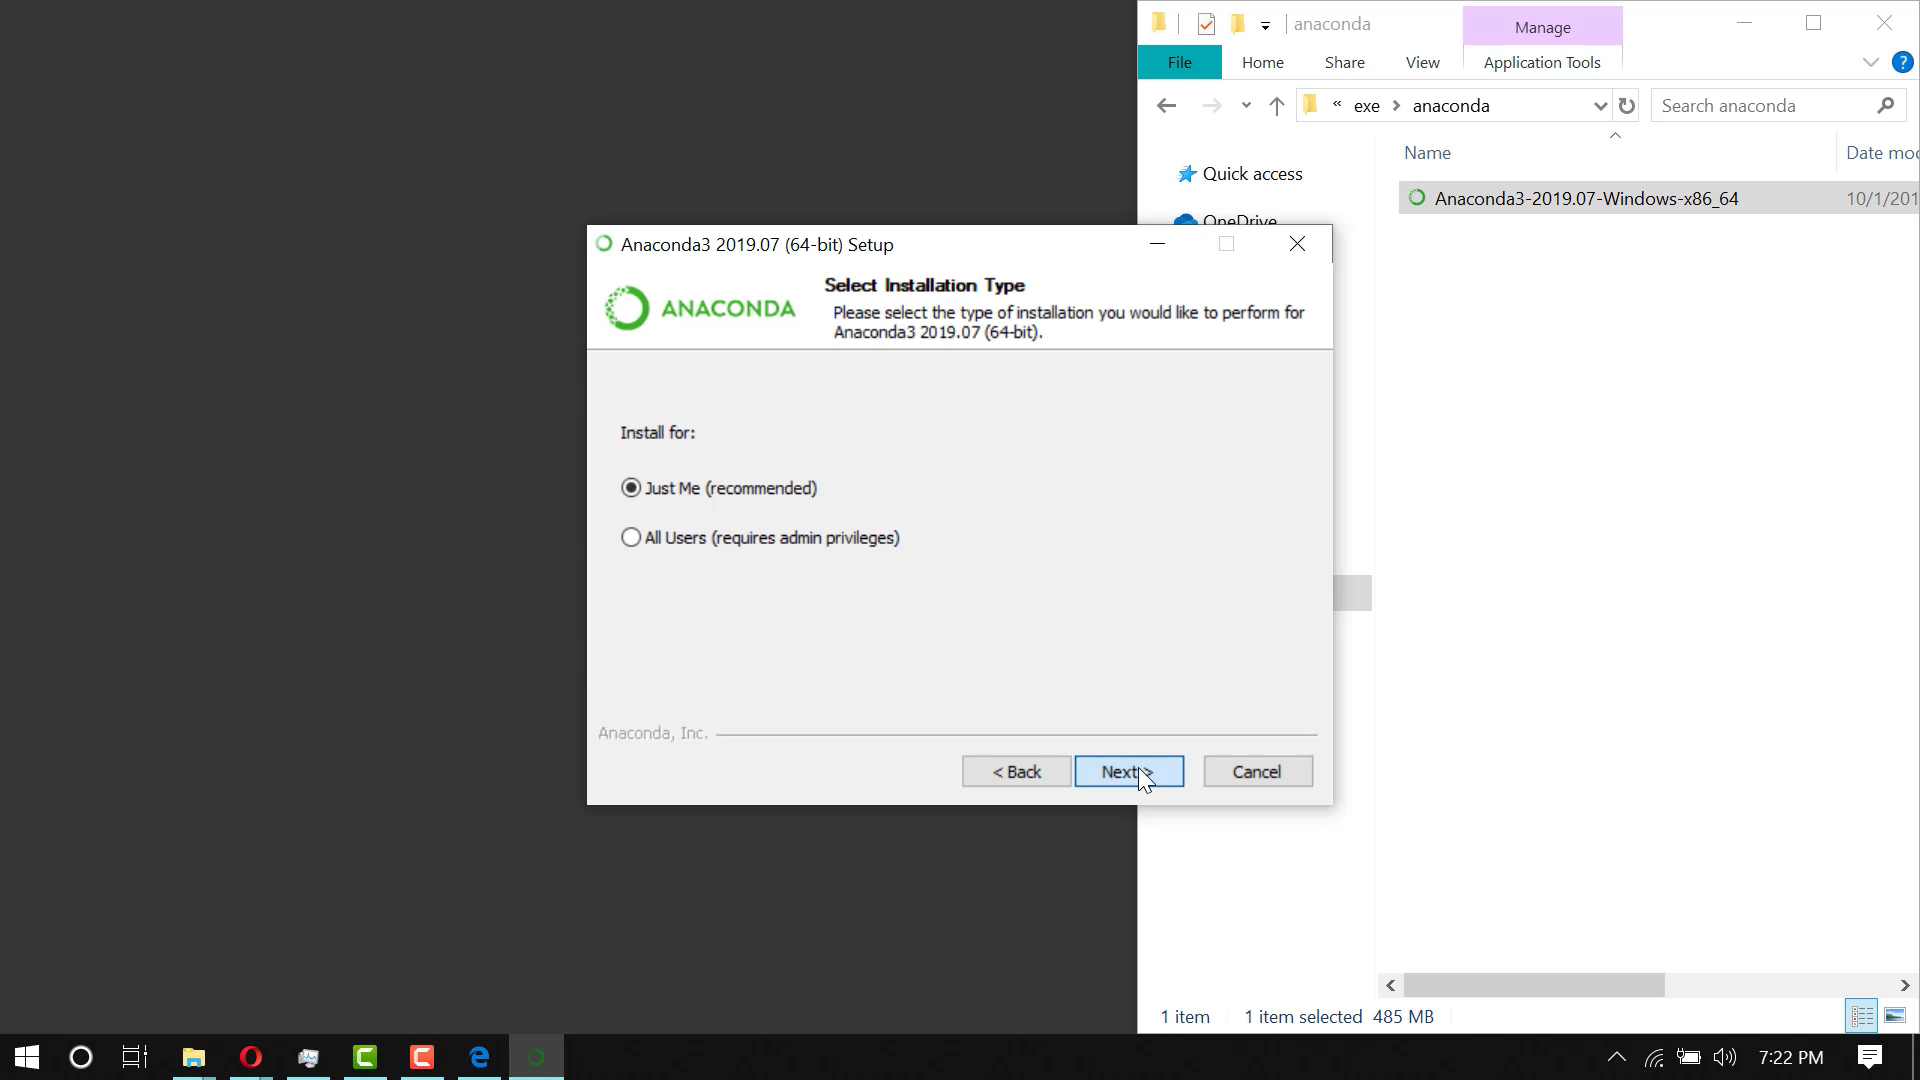
\includegraphics[width=7.5cm]{gambar/anaconda/Screenshot (62).png} 
	\item Tentukan lokasi folder dimana anaconda akan di install lalu klik "next"\\
	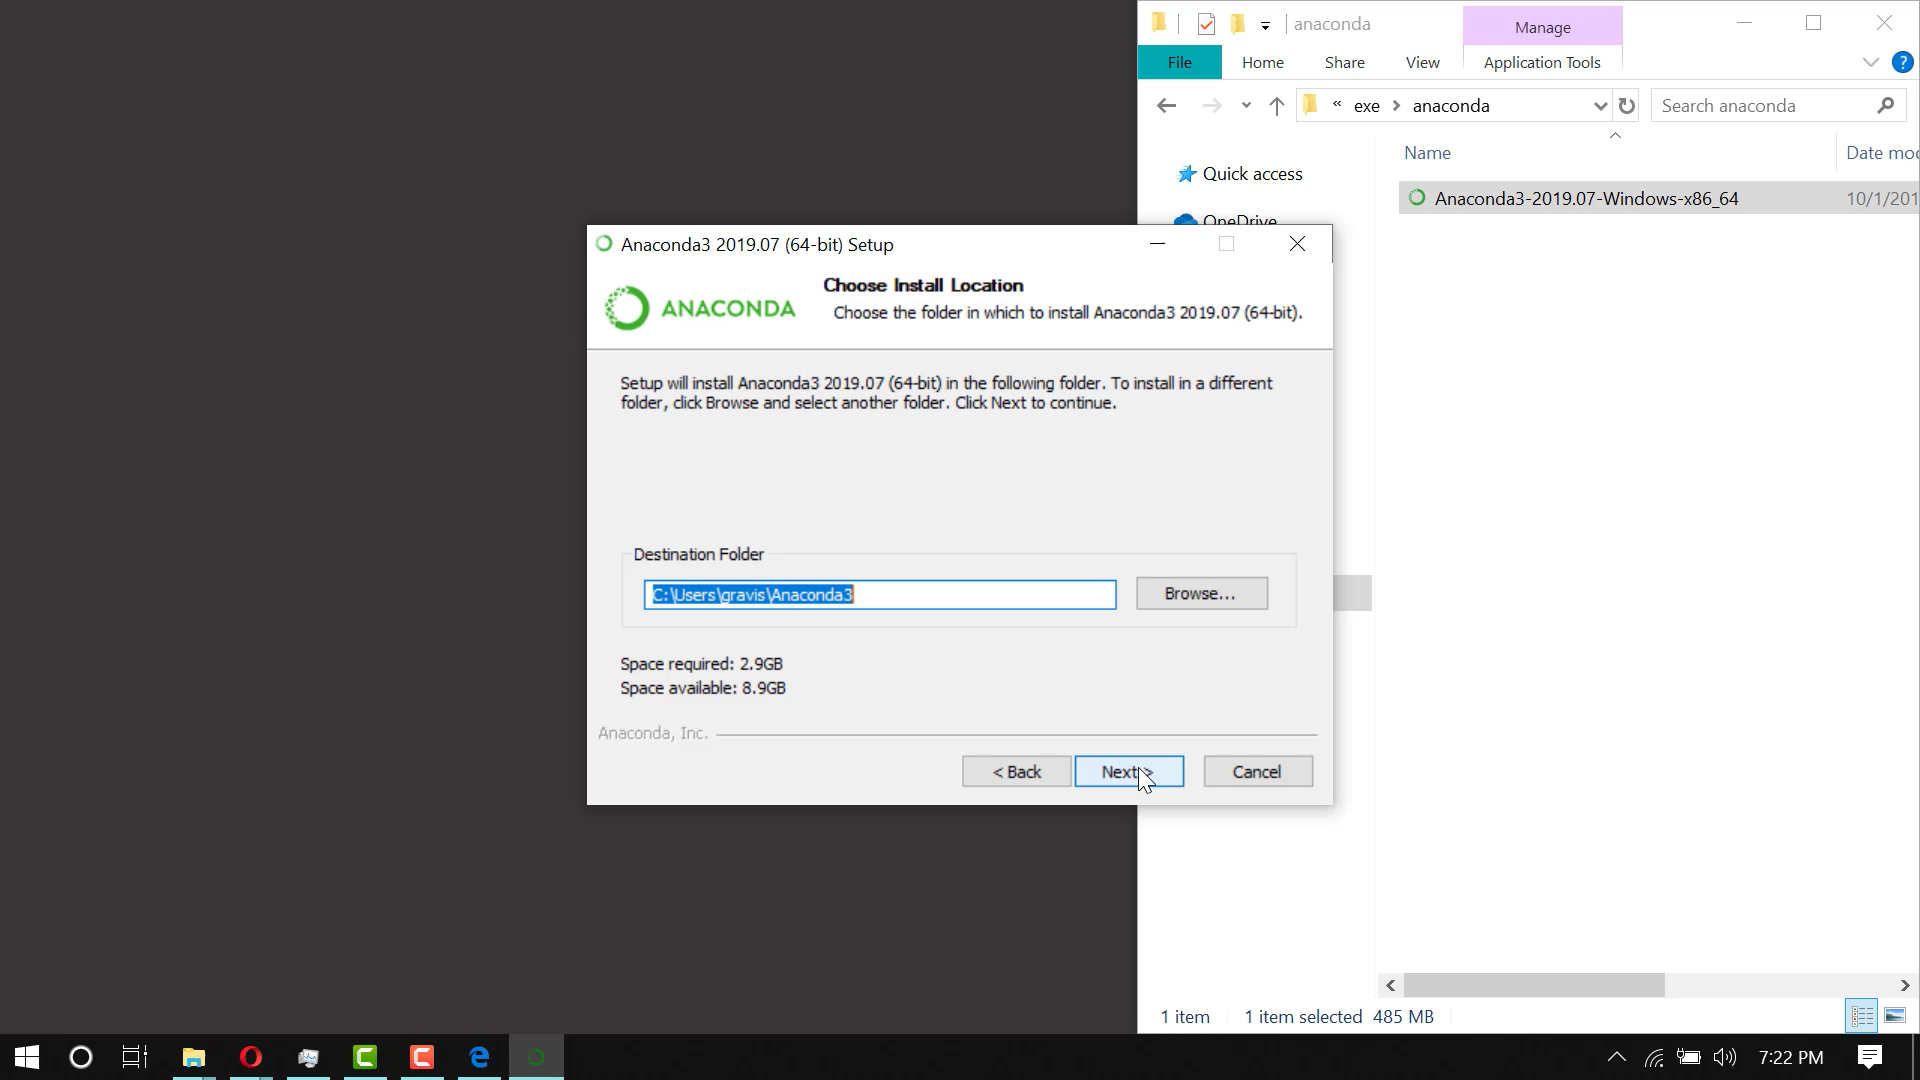
\includegraphics[width=7.5cm]{gambar/anaconda/Screenshot (63).png} 
	\item Klik cetang pada "Add anaconda to my PATH environment variable" lalu klik "next"\\
	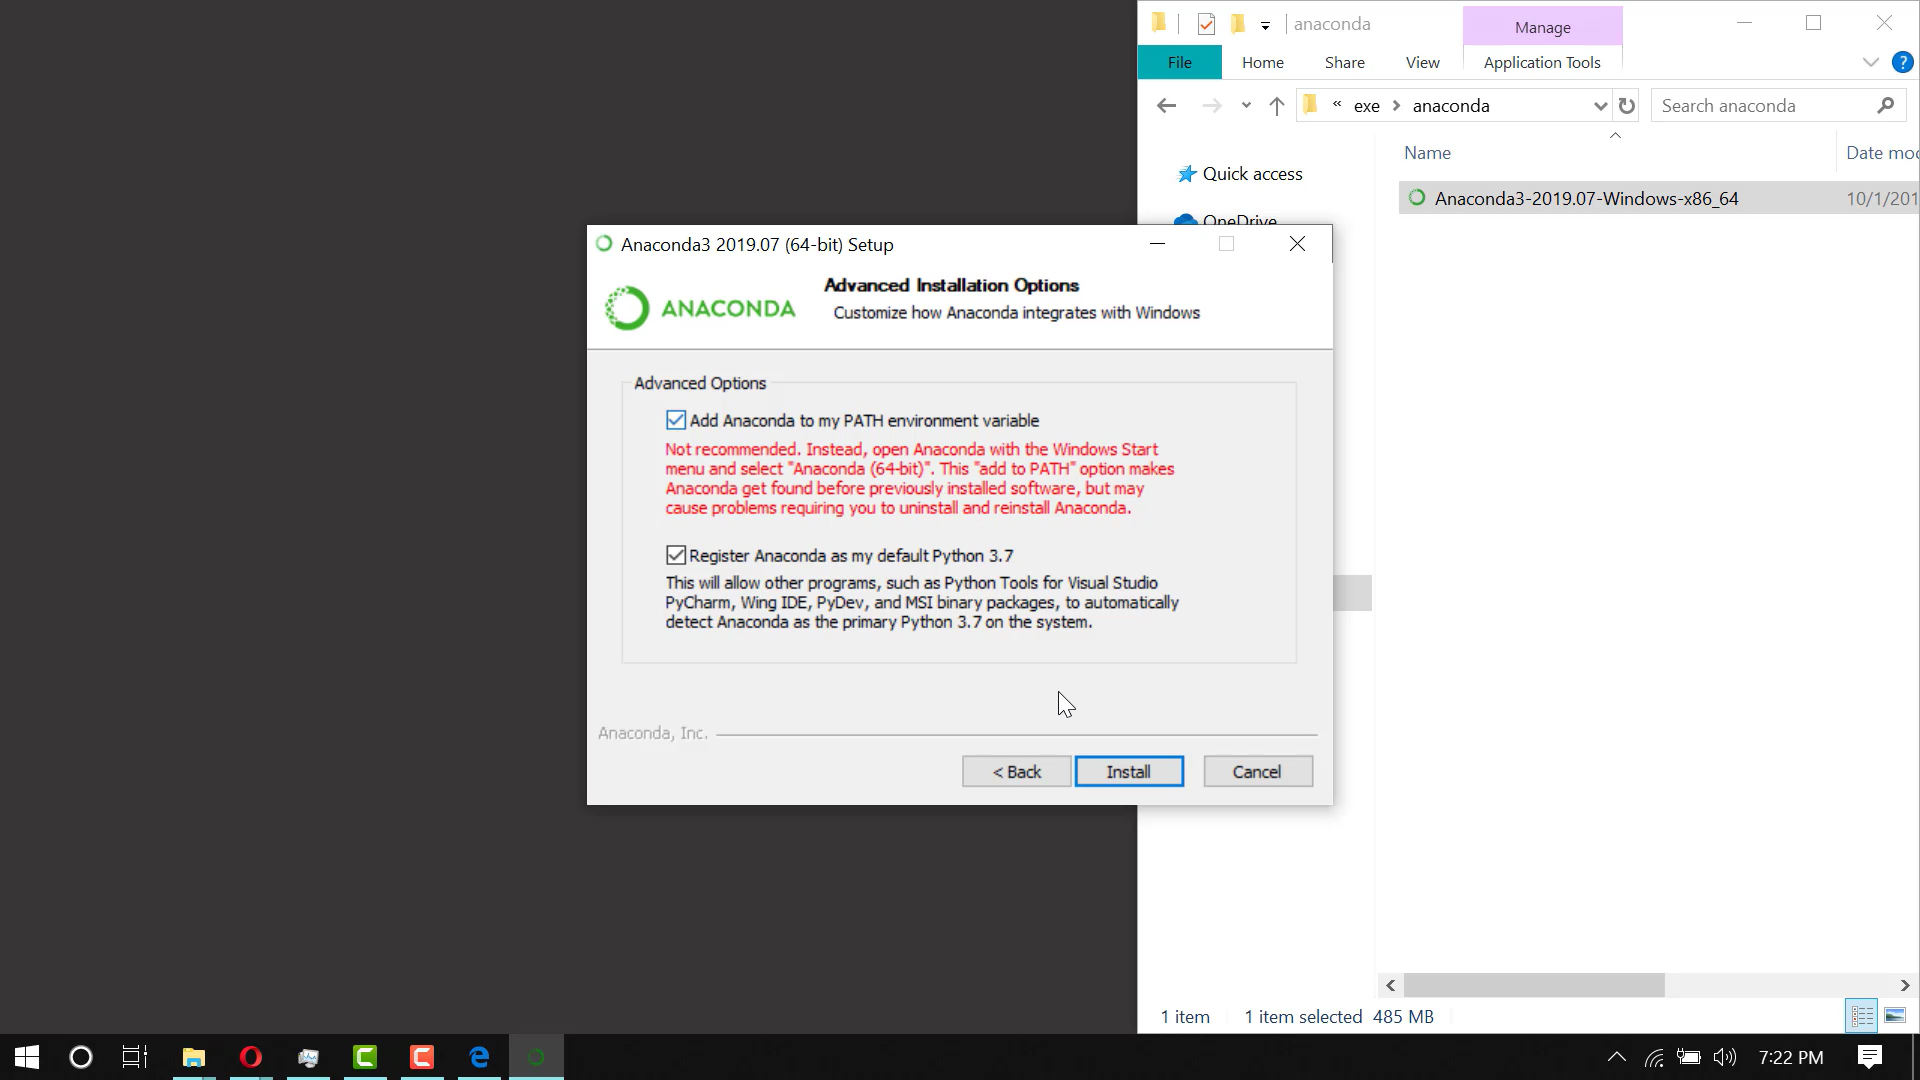
\includegraphics[width=7.5cm]{gambar/anaconda/Screenshot (66).png} 
	\item Tunggu hingga proses selesai lalu klik "next"\\
	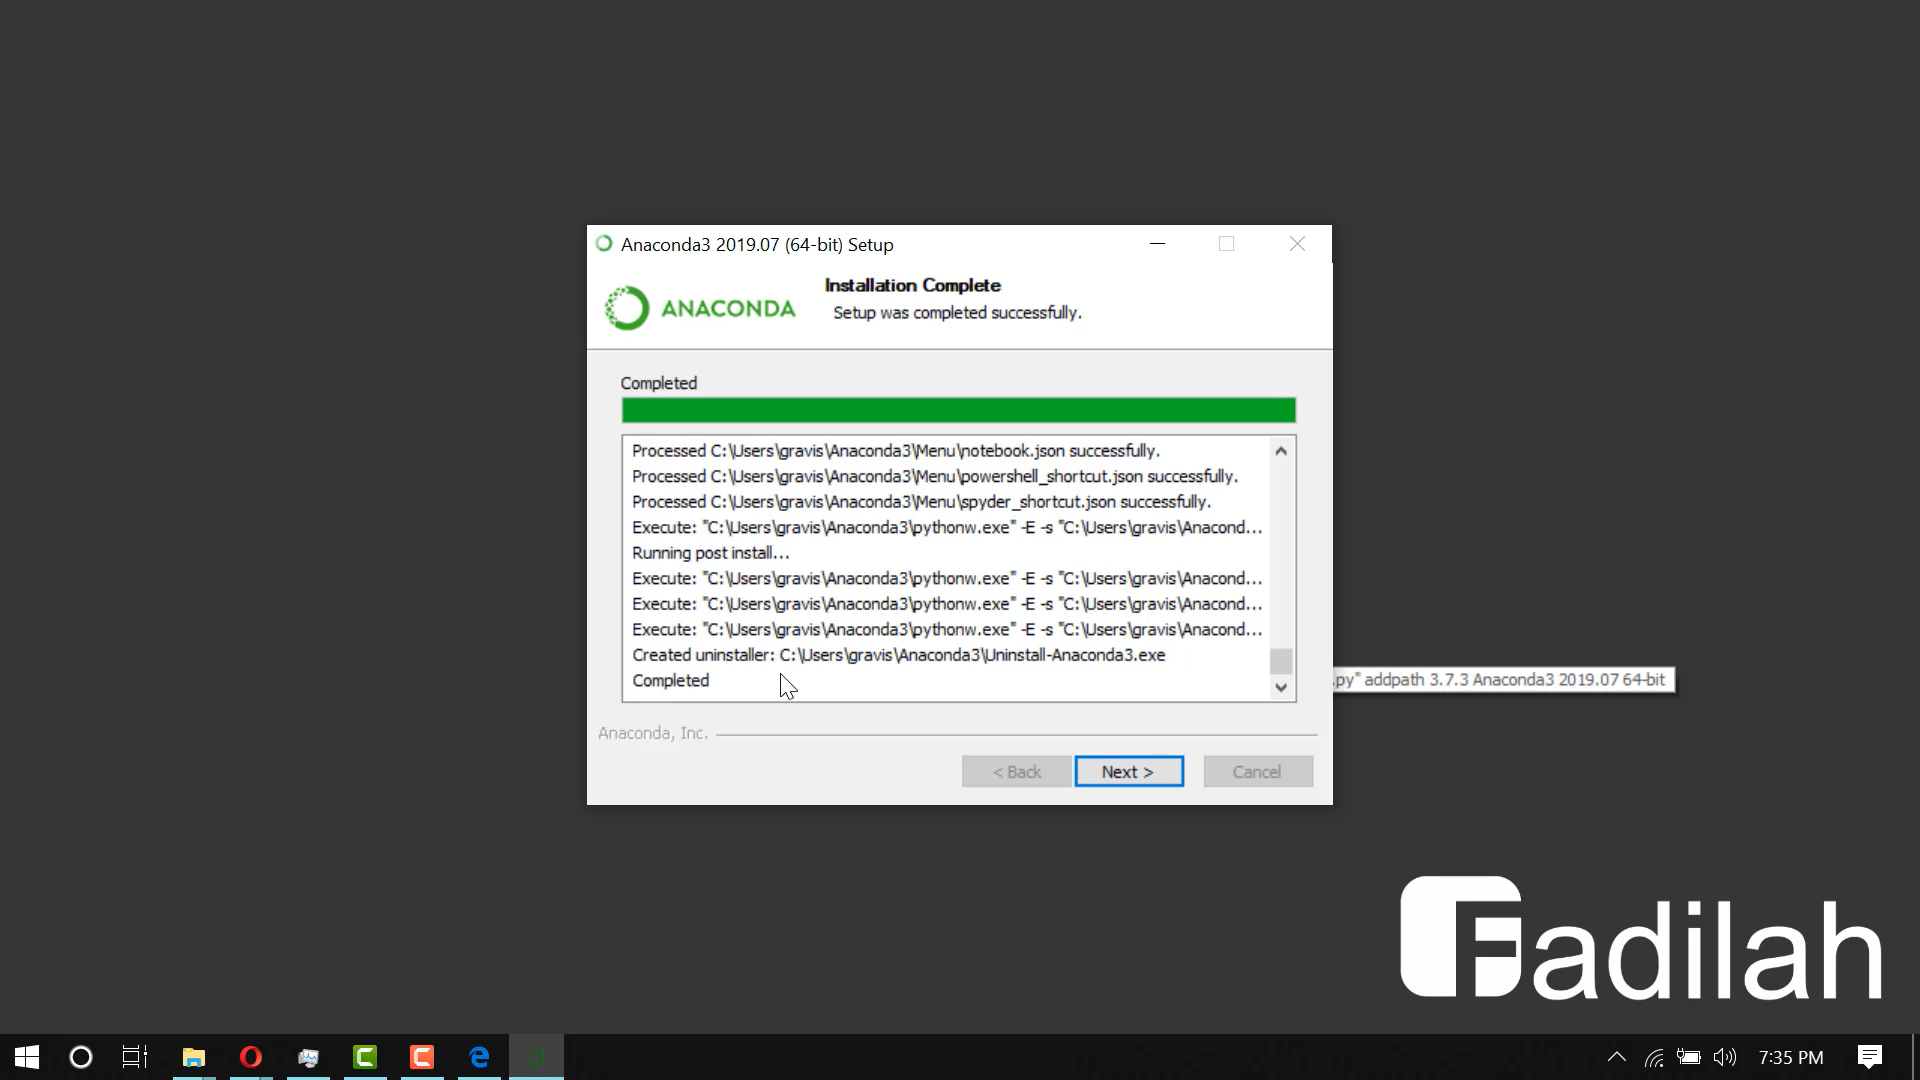
\includegraphics[width=7.5cm]{gambar/anaconda/Screenshot (93).png} 
	\item Klik "next"\\
	 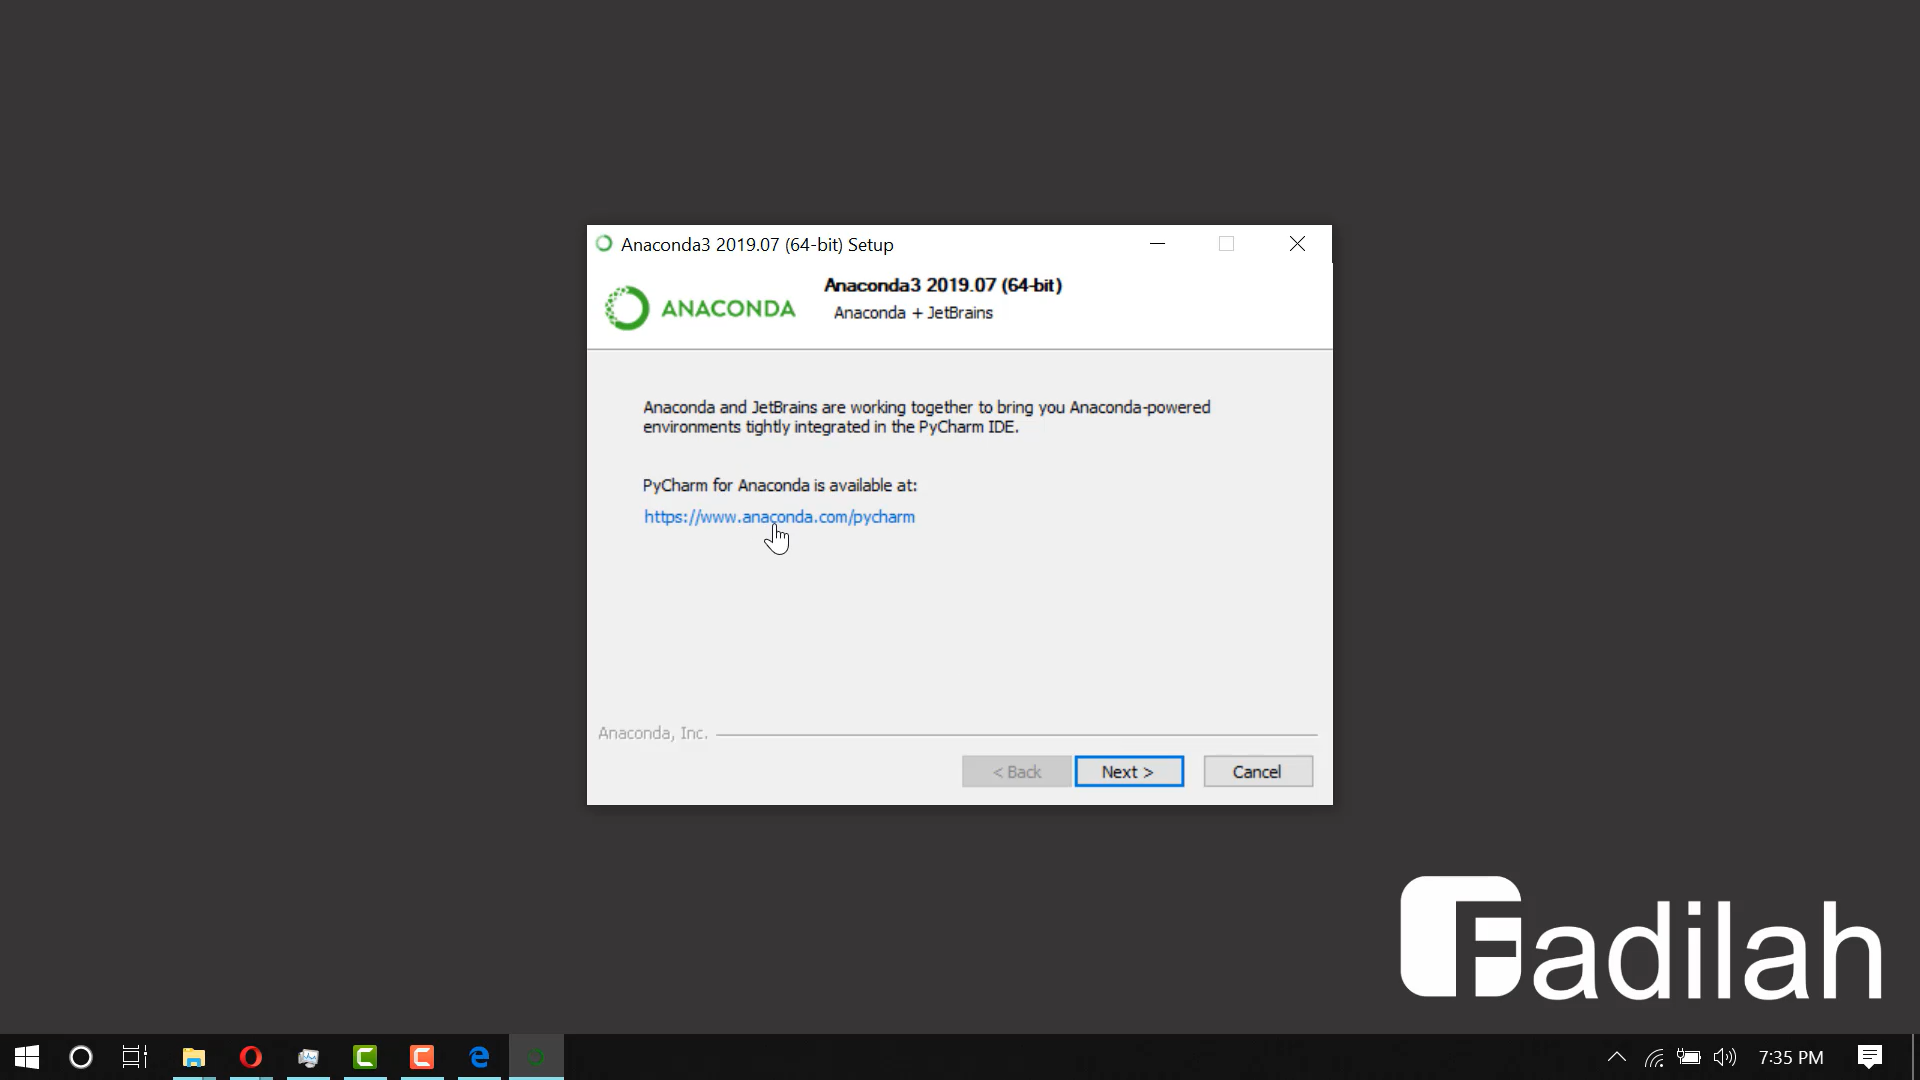
\includegraphics[width=7.5cm]{gambar/anaconda/Screenshot (96).png} 
	\item Klik "finish"\\
	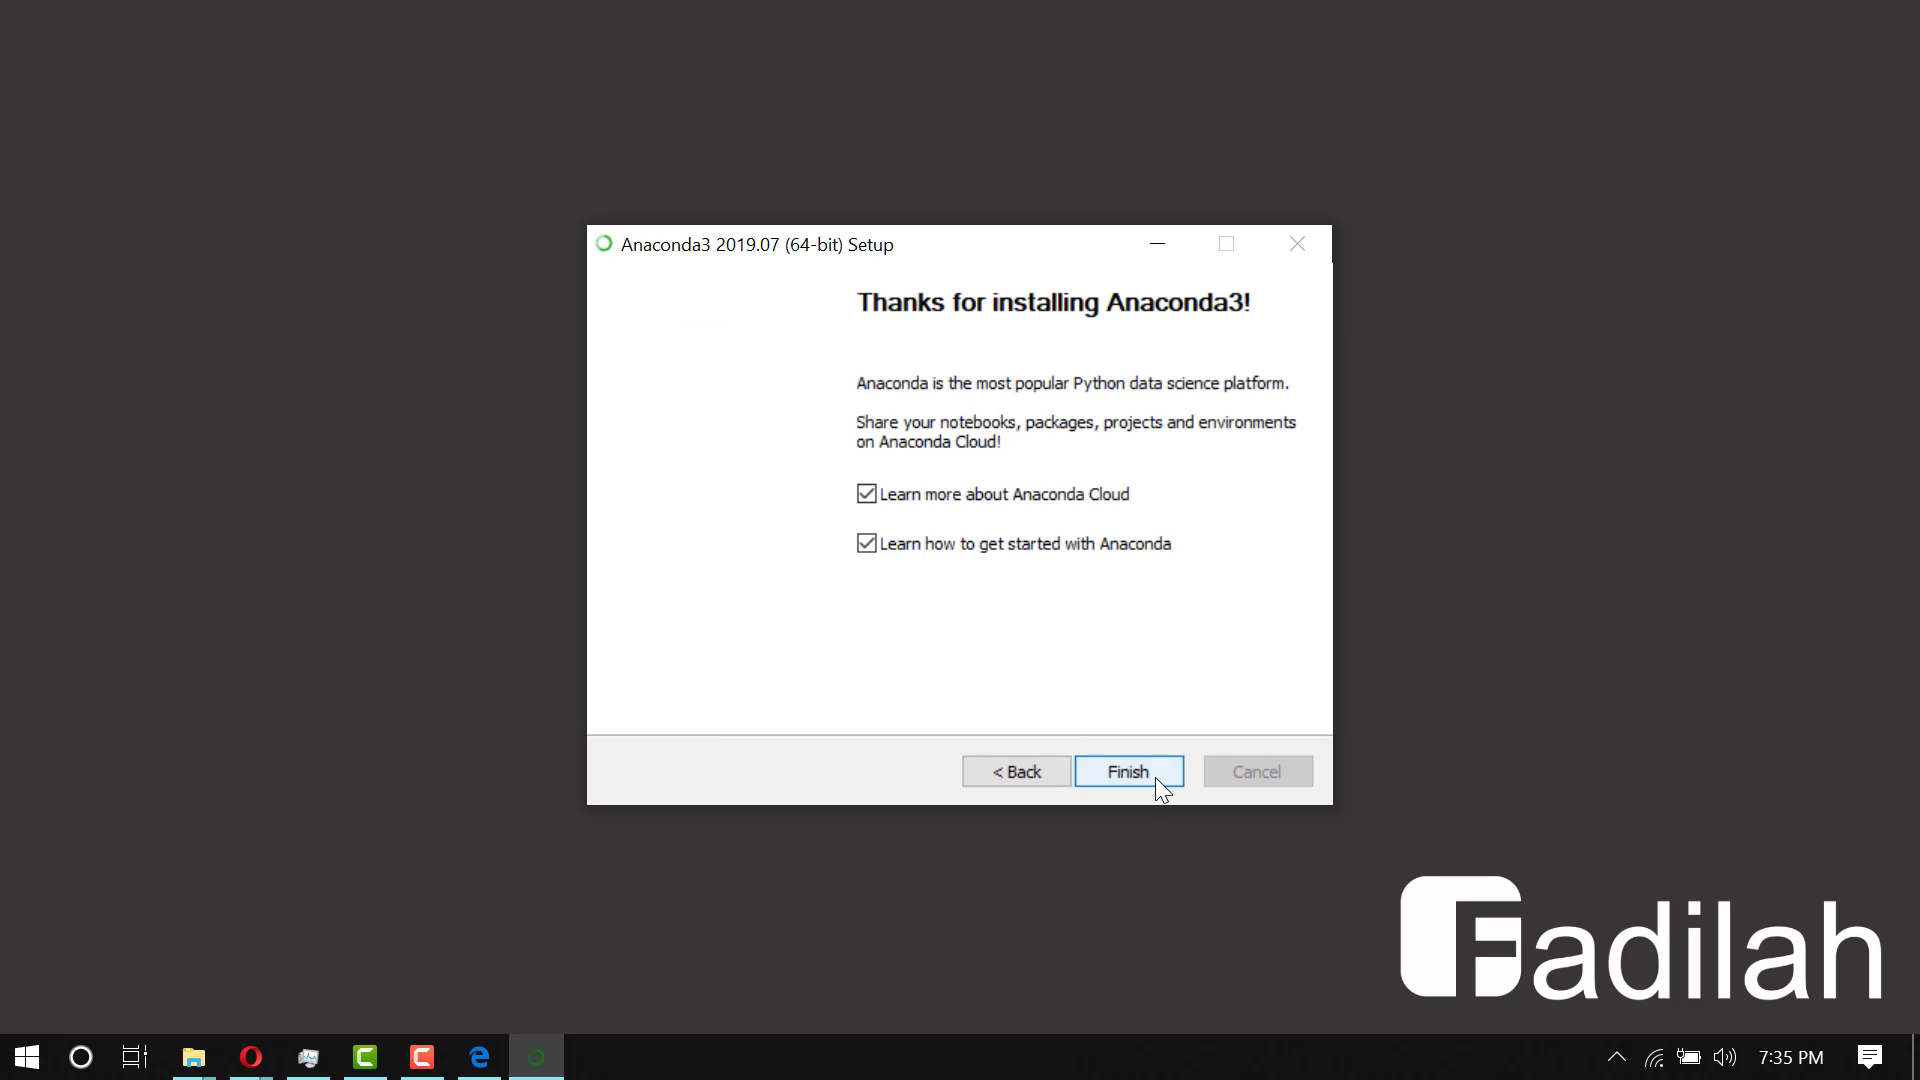
\includegraphics[width=7.5cm]{gambar/anaconda/Screenshot (95).png} 
\end{itemize}

\section{update anaconda \& environment}
\paragraph{} 
\begin{itemize}
	\item Buka Anaconda navigator\\
	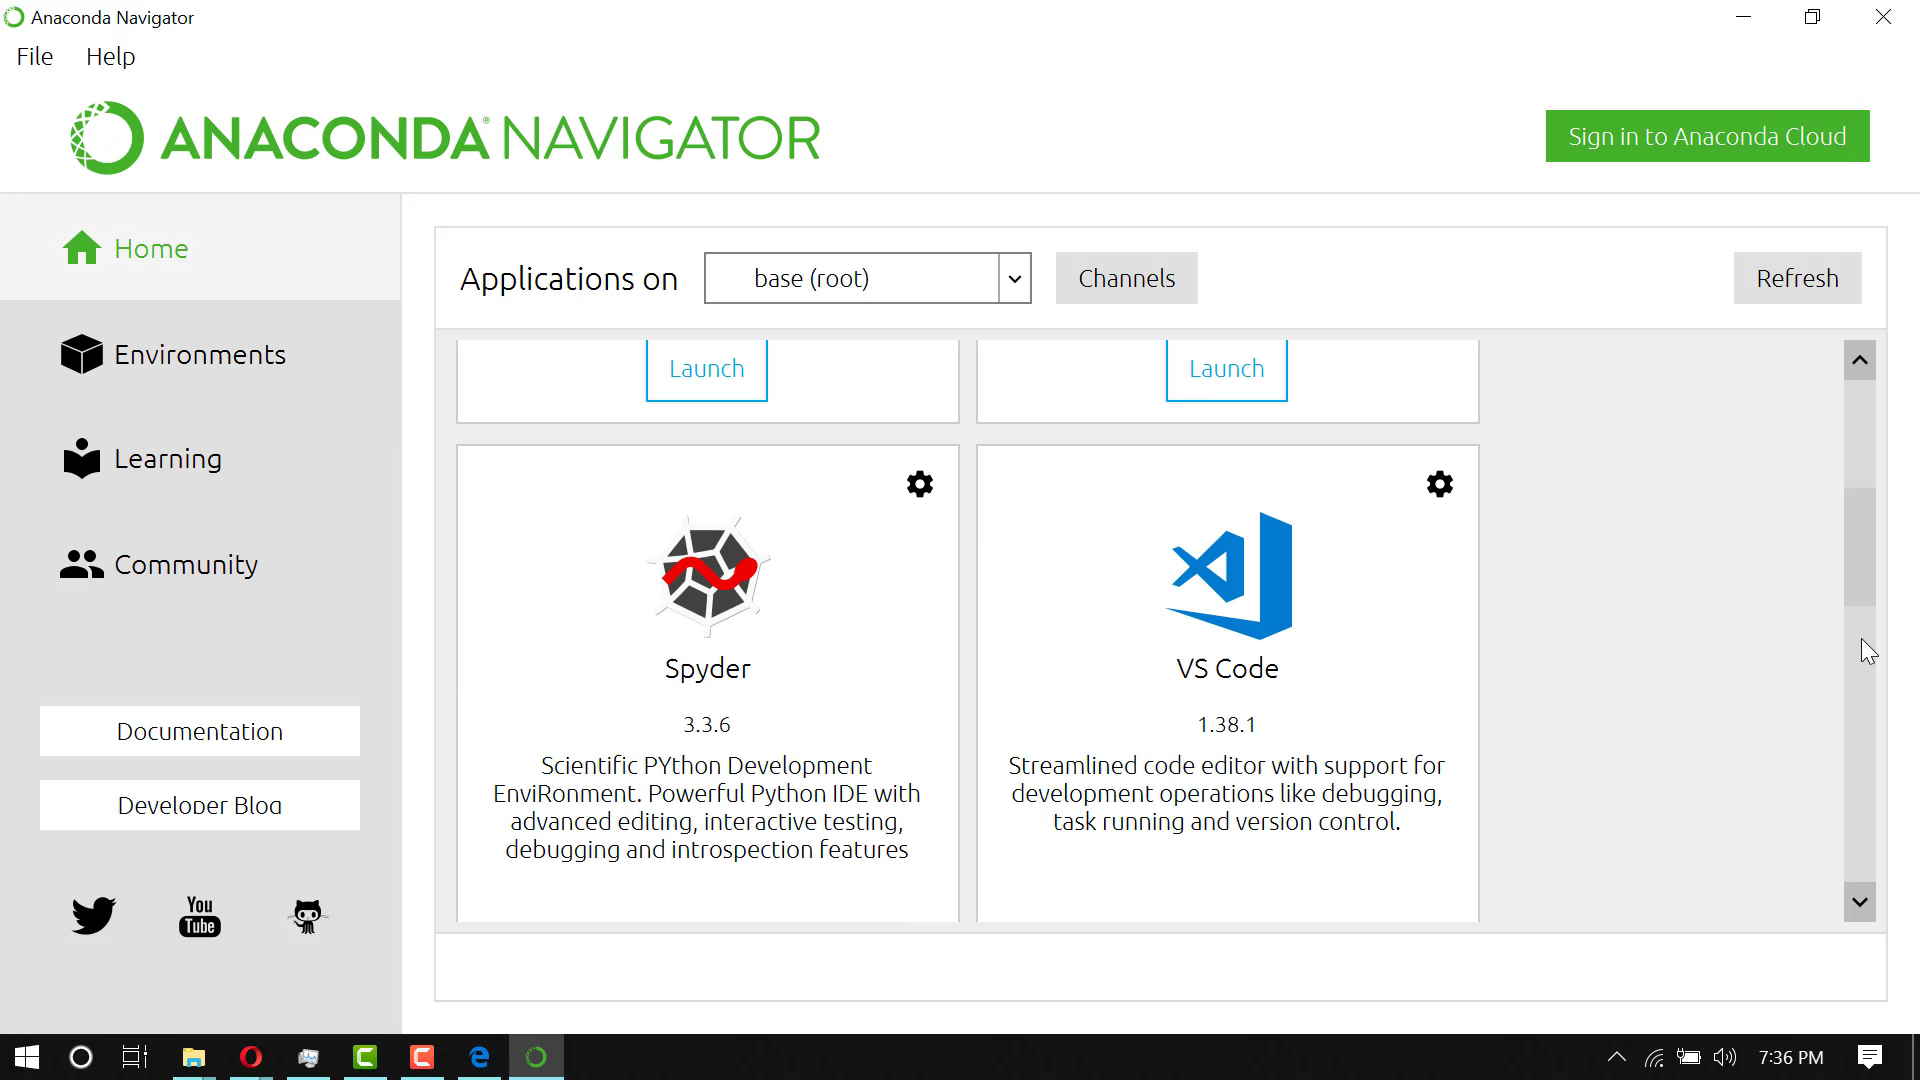
\includegraphics[width=7.5cm]{gambar/update anaconda/Screenshot (72).png} 
	\item Buka Pilih menu "Environment", cari "anaconda"\\
	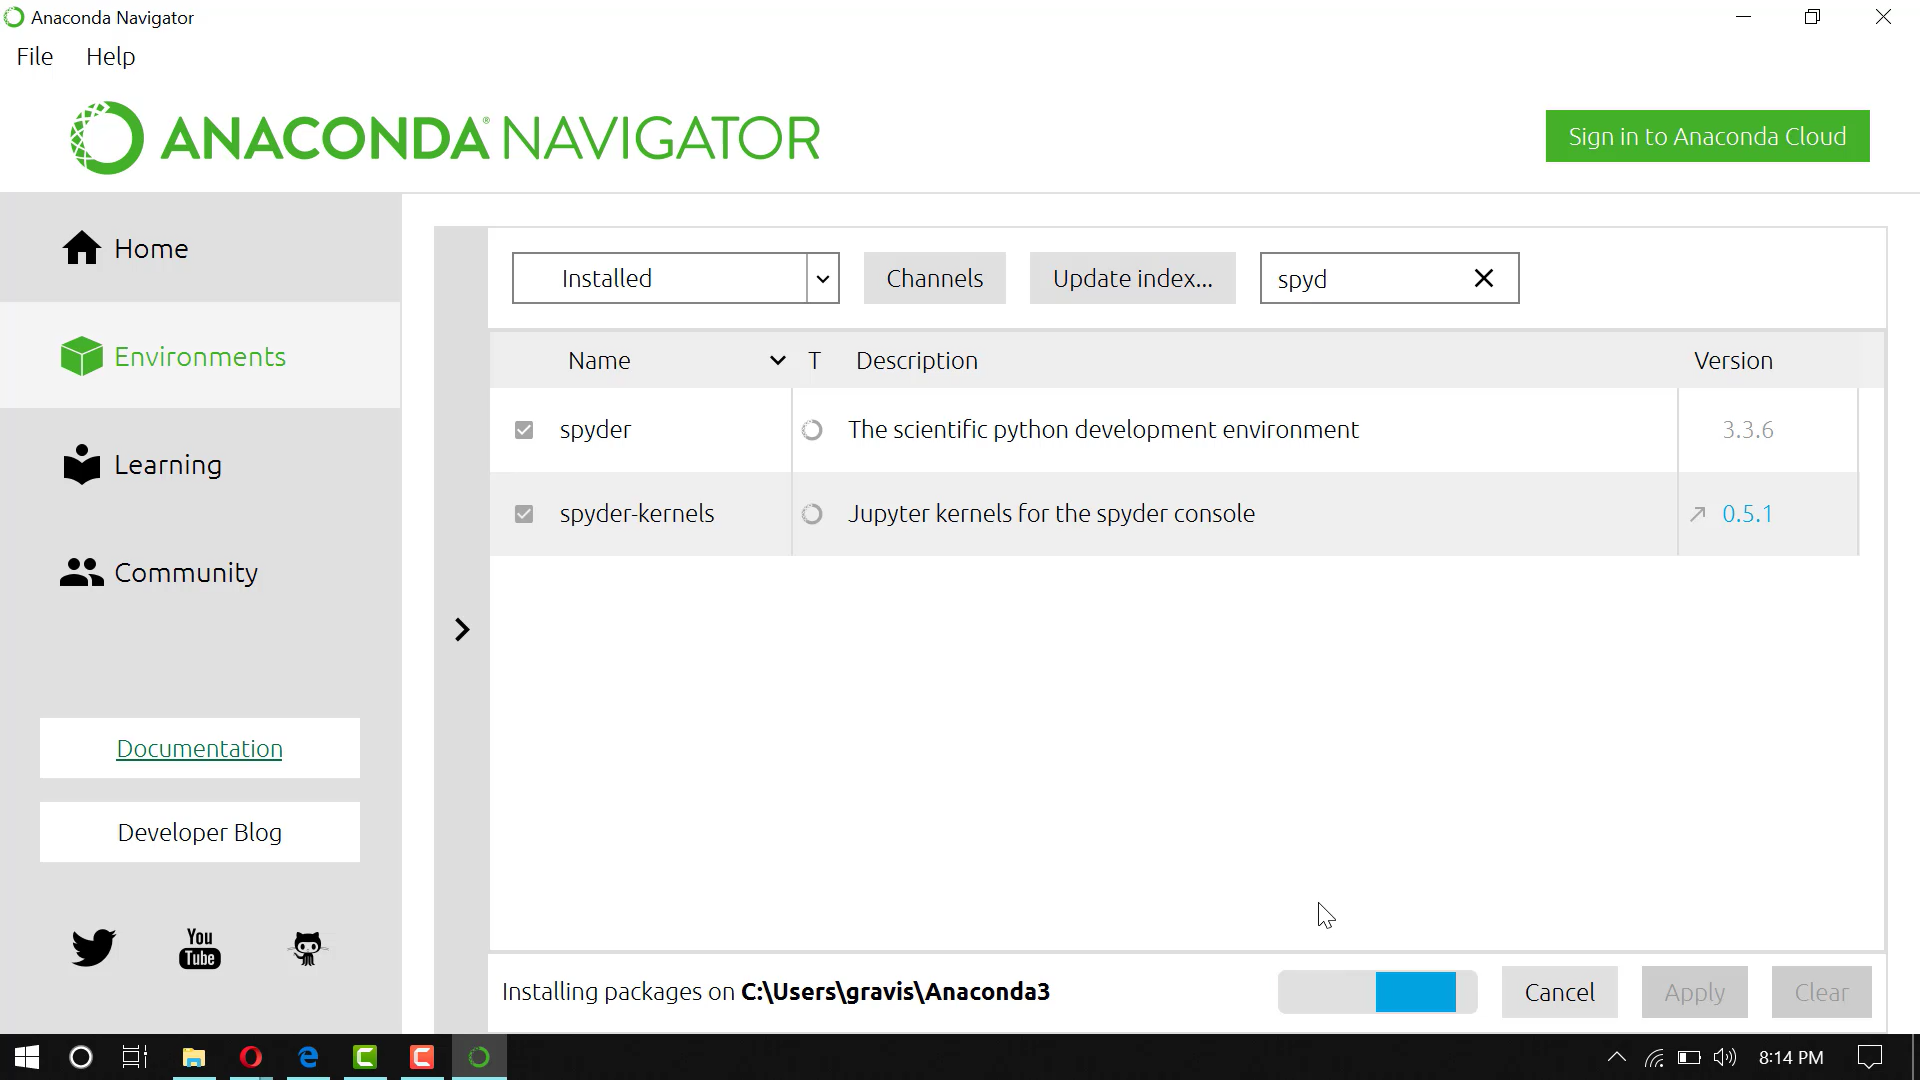
\includegraphics[width=7.5cm]{gambar/update anaconda/Screenshot (74).png} 
	\item Klik cetang hijau, pilih "mark for spesific version installation", lalu pilih versi terbaru\\
	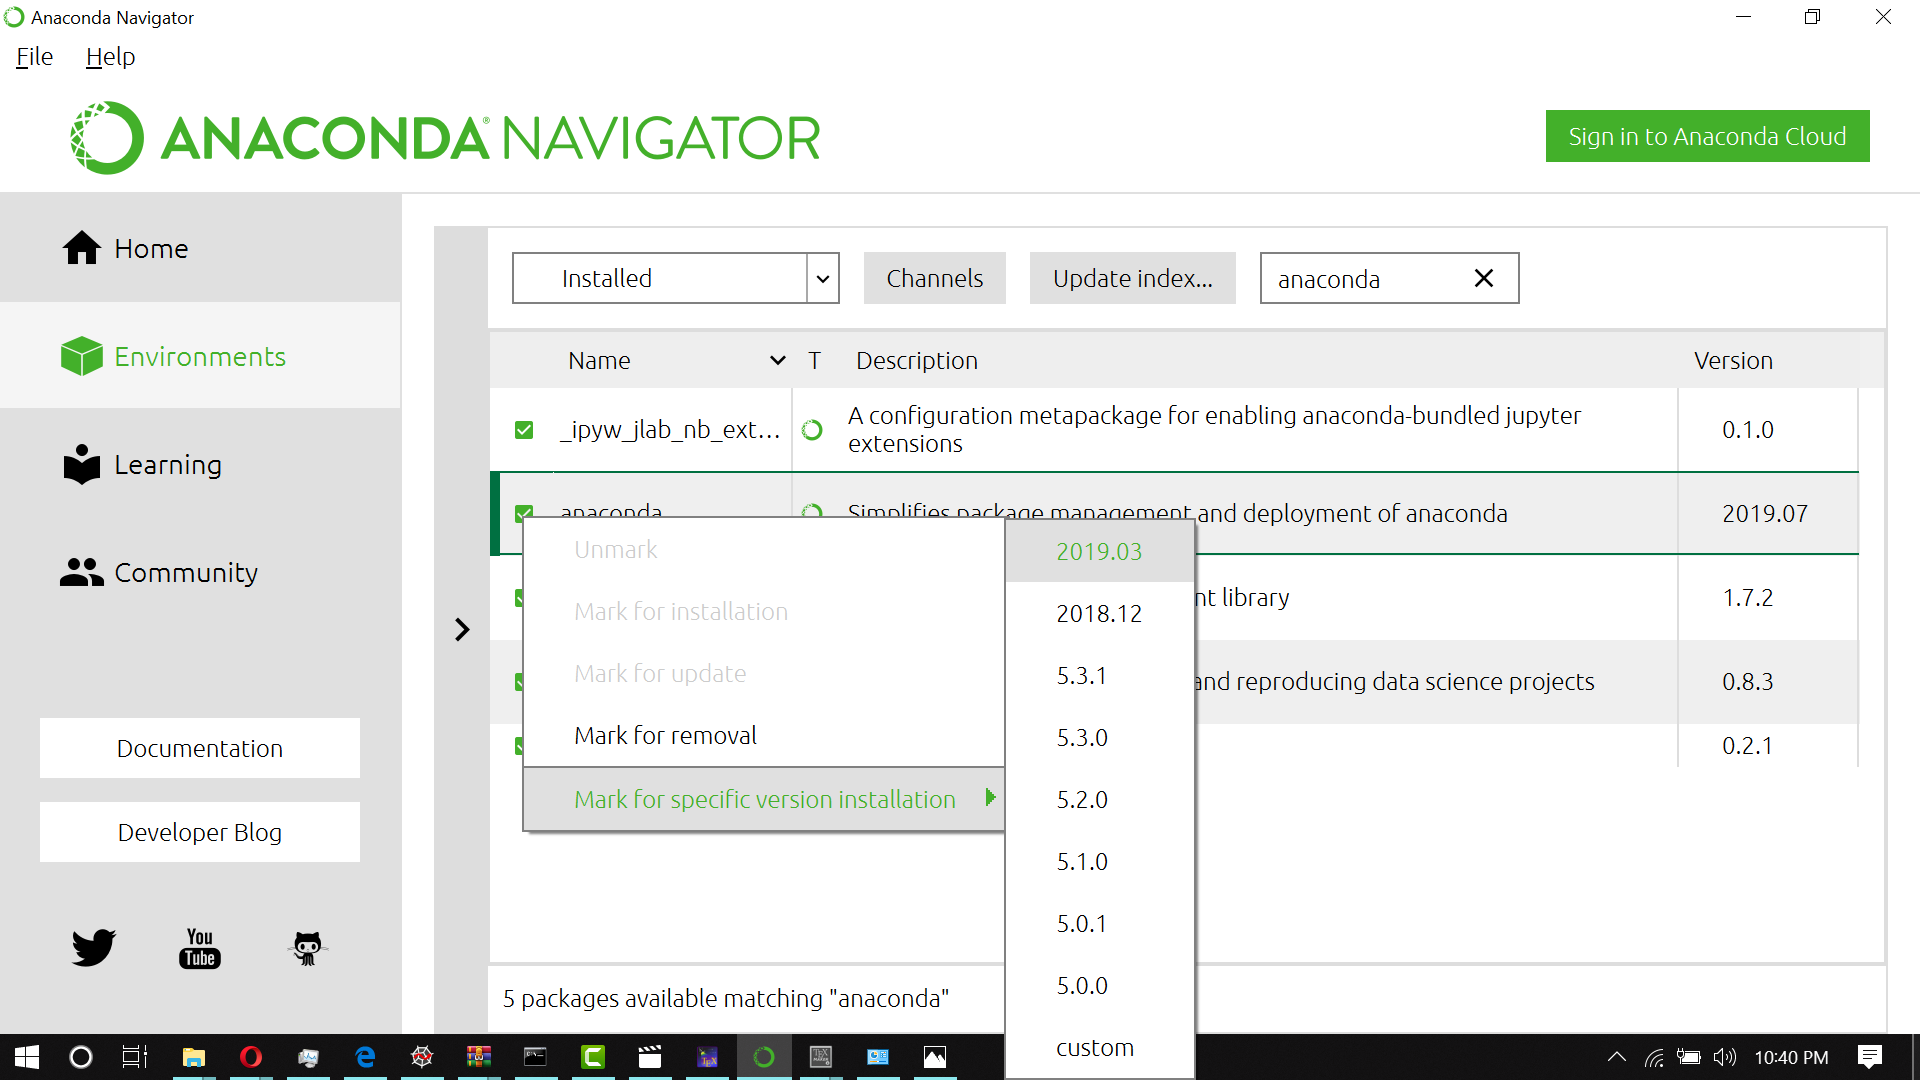
\includegraphics[width=7.5cm]{gambar/update anaconda/Screenshot (97).png} 
	\item klik "apply" dan tunggu hingga selesai\\
	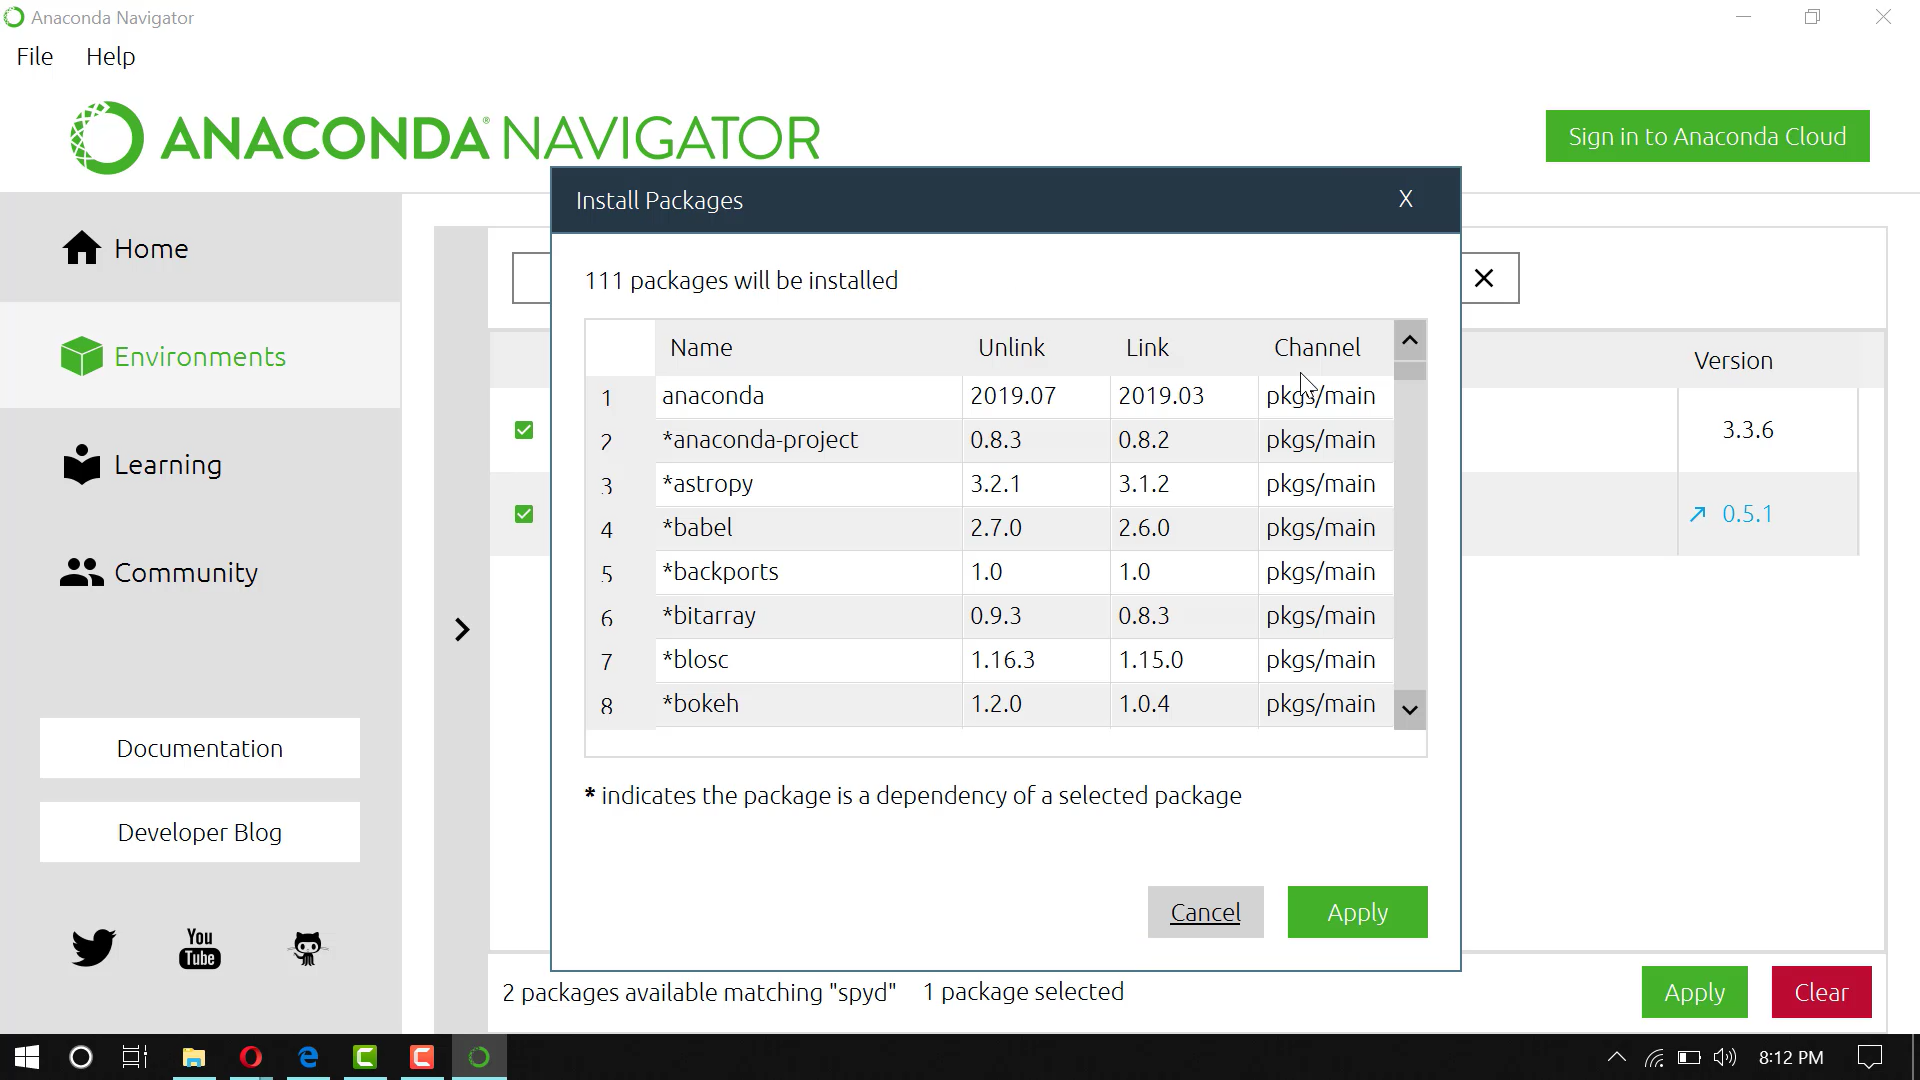
\includegraphics[width=7.5cm]{gambar/update anaconda/Screenshot (73).png} 
\end{itemize}

\section{instalasi pip}
\paragraph{}
\begin{itemize}
	\item Buka website : https://bootstrap.pypa.io/get-pip.py\\
	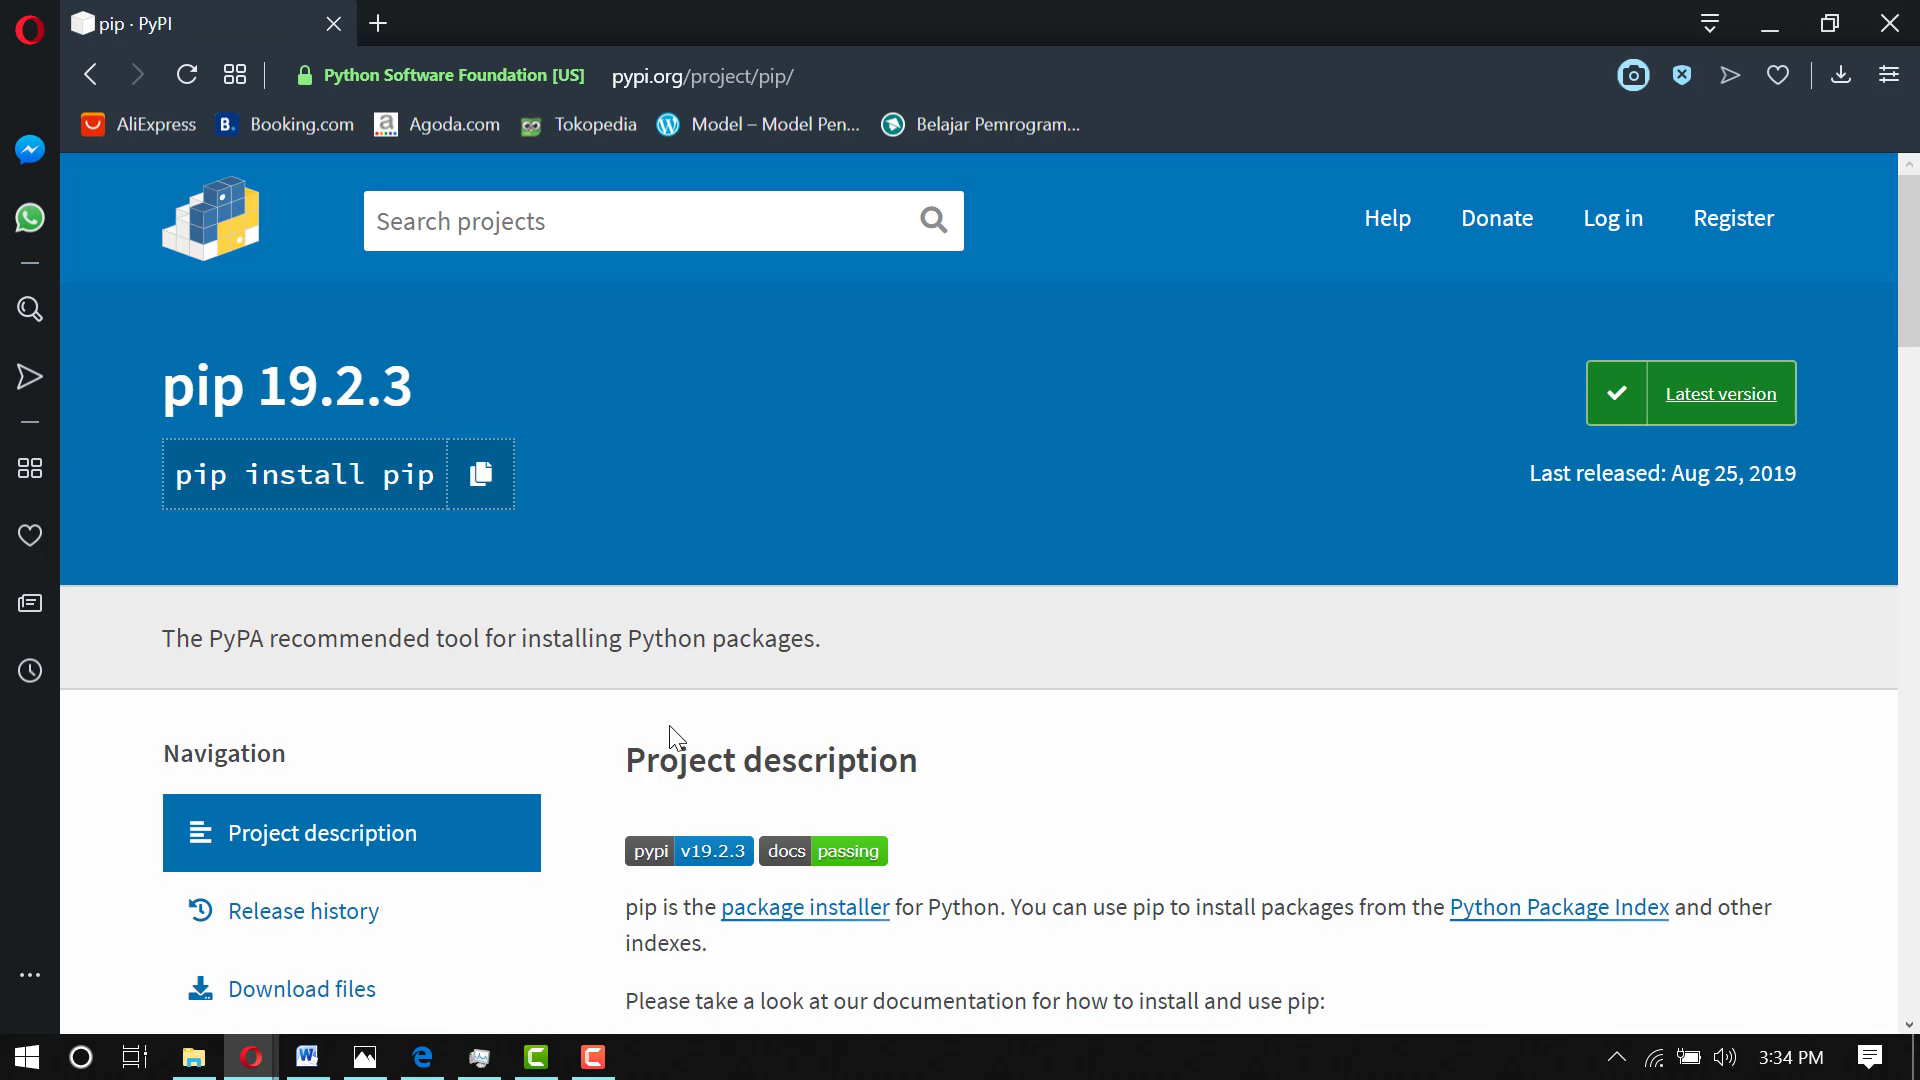
\includegraphics[width=7.5cm]{gambar/pip/Screenshot (76).png} 
	\item Klik kanan "save as .."  lalu klik "save"\\
	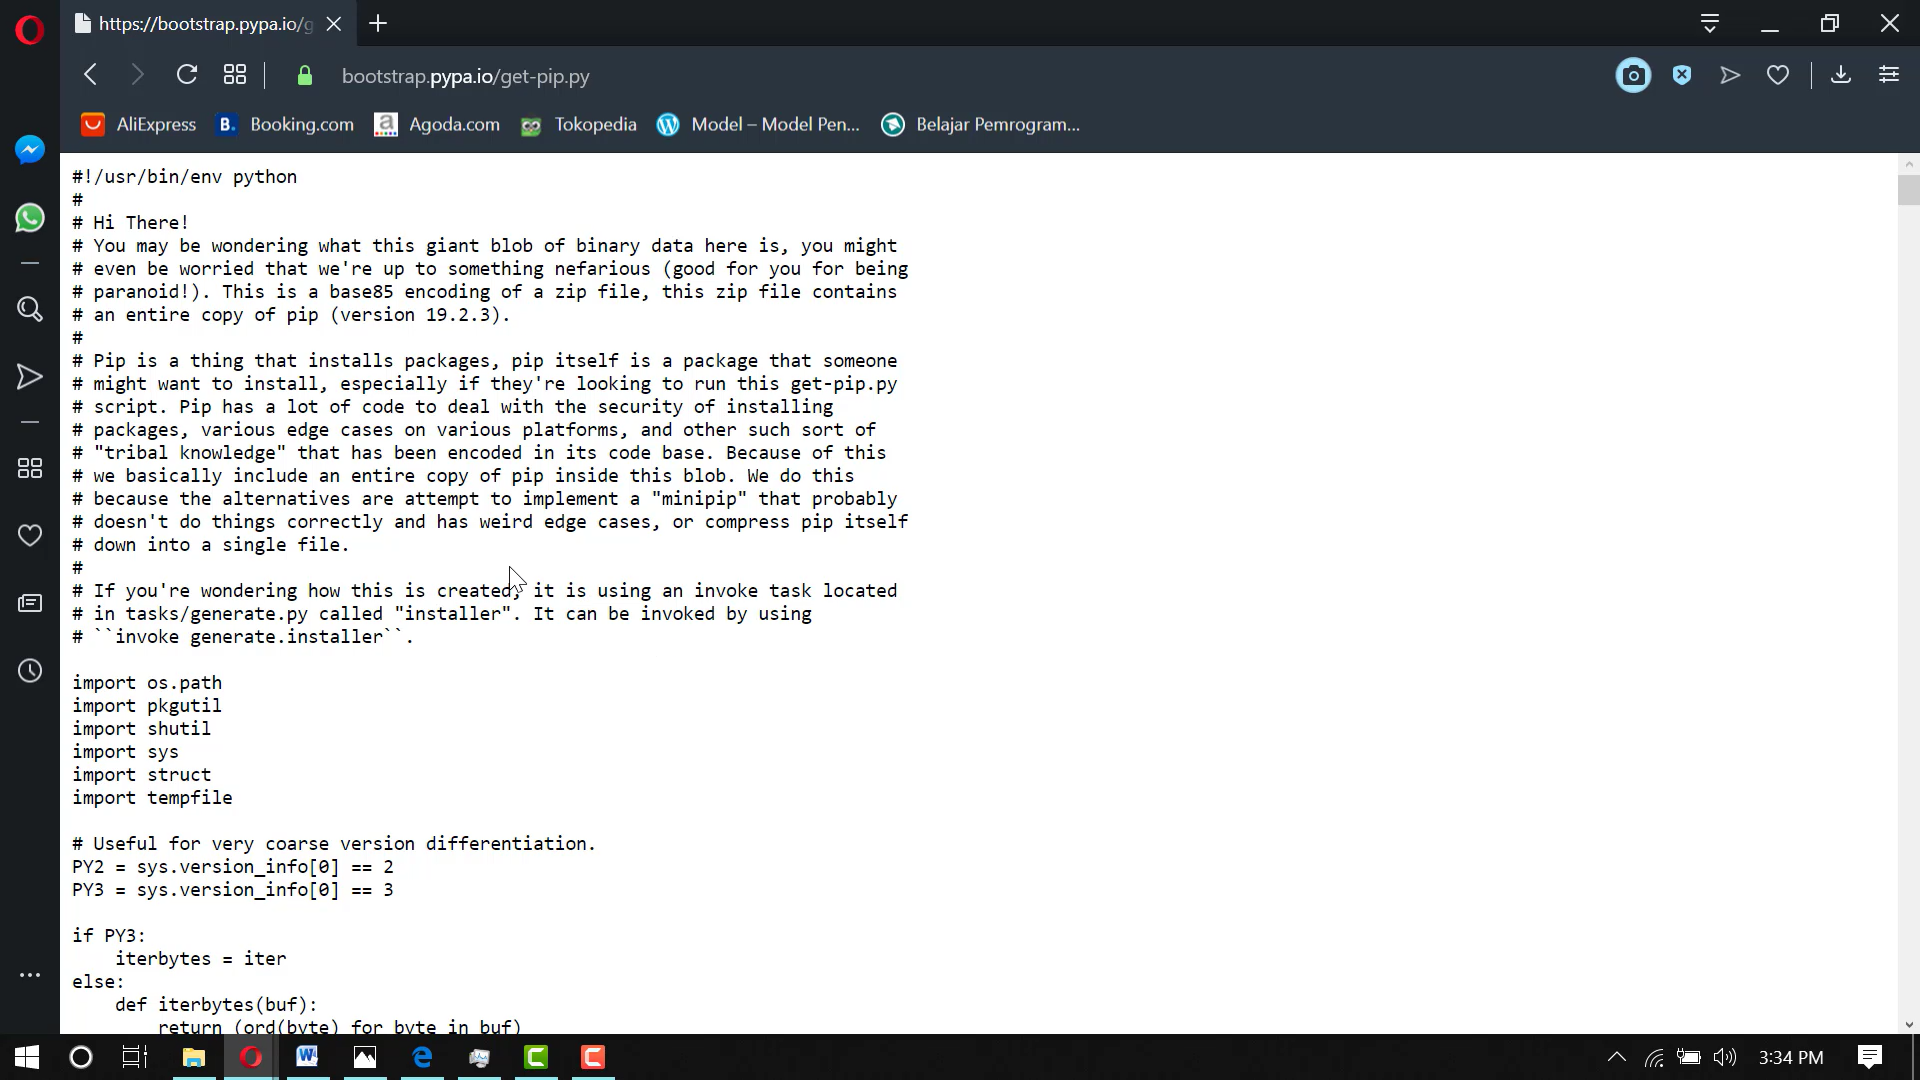
\includegraphics[width=7.5cm]{gambar/pip/Screenshot (77).png} 
	\item Buka Command prompt, masuk ke directori dimana file di install, lalu ketik "python namafile.py"\\
	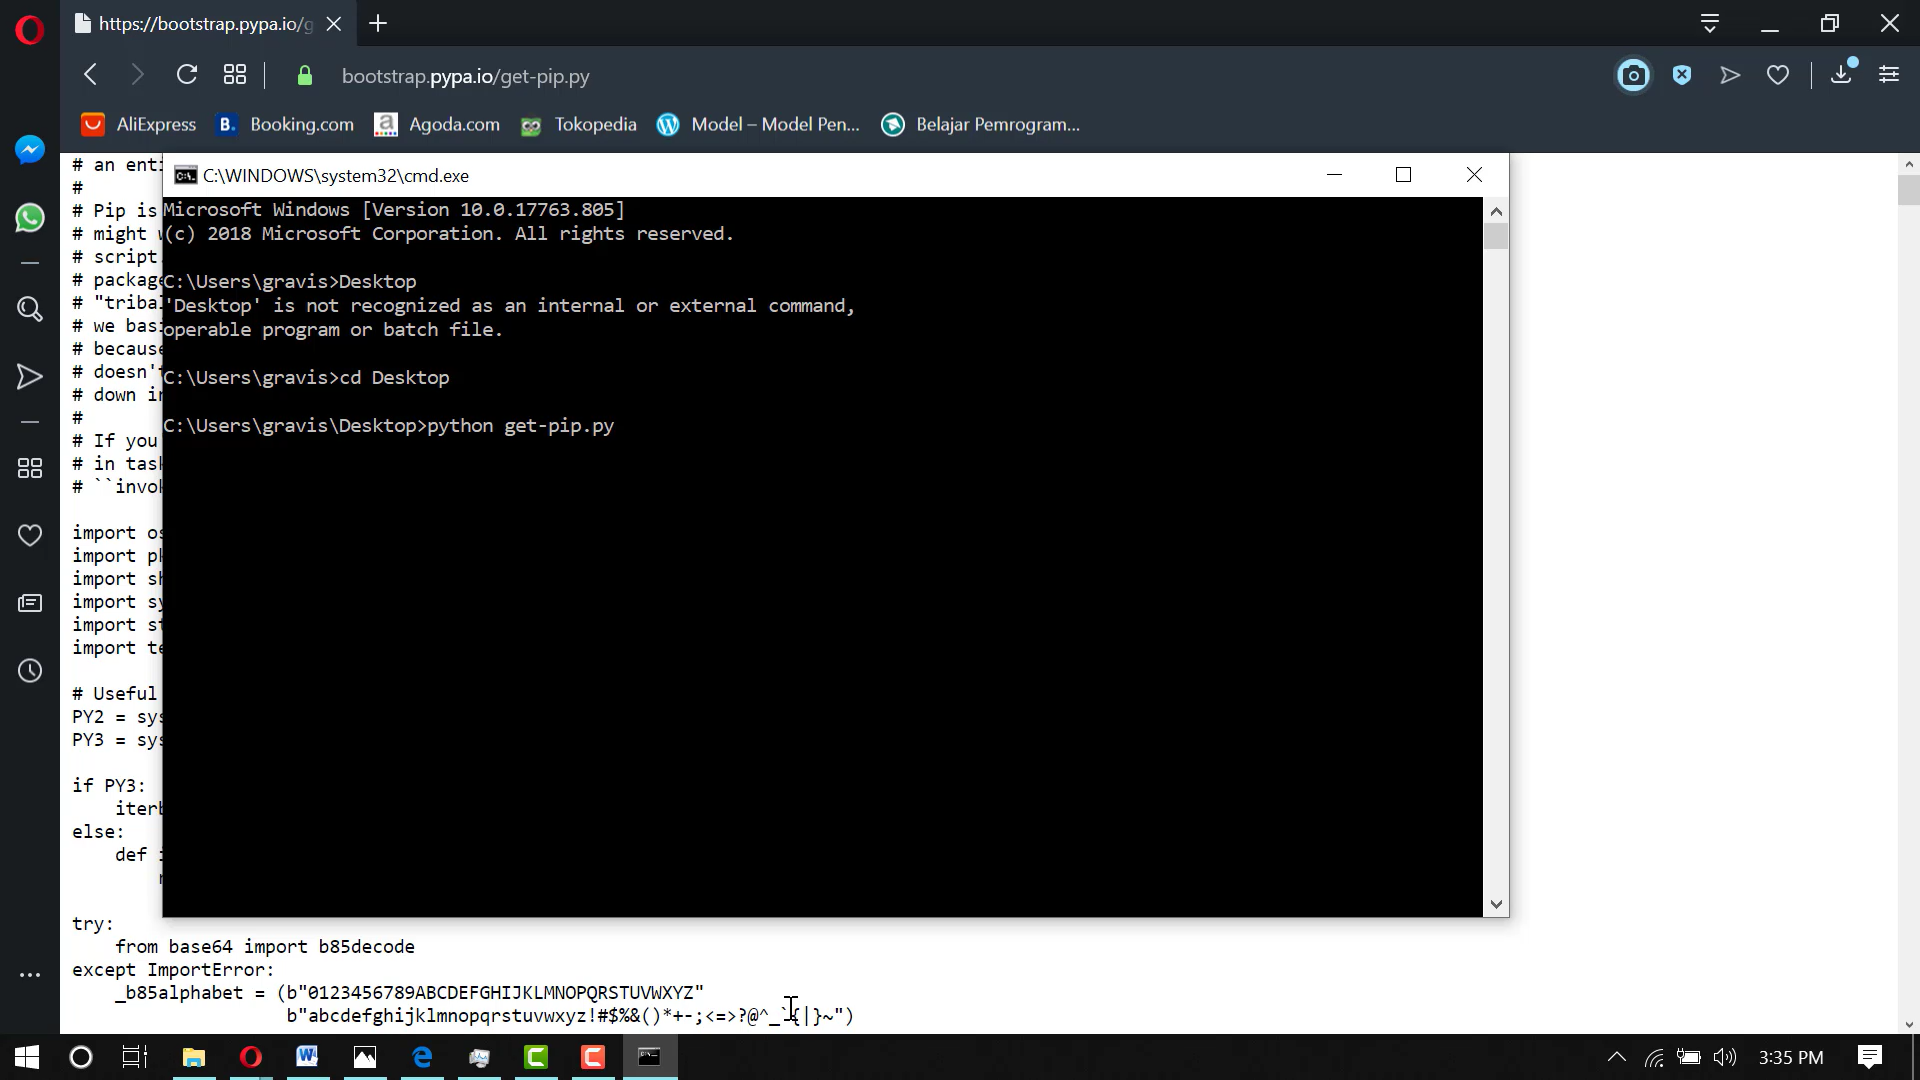
\includegraphics[width=7.5cm]{gambar/pip/Screenshot (78).png} 
	\item Tunggu hingga selesai\\
	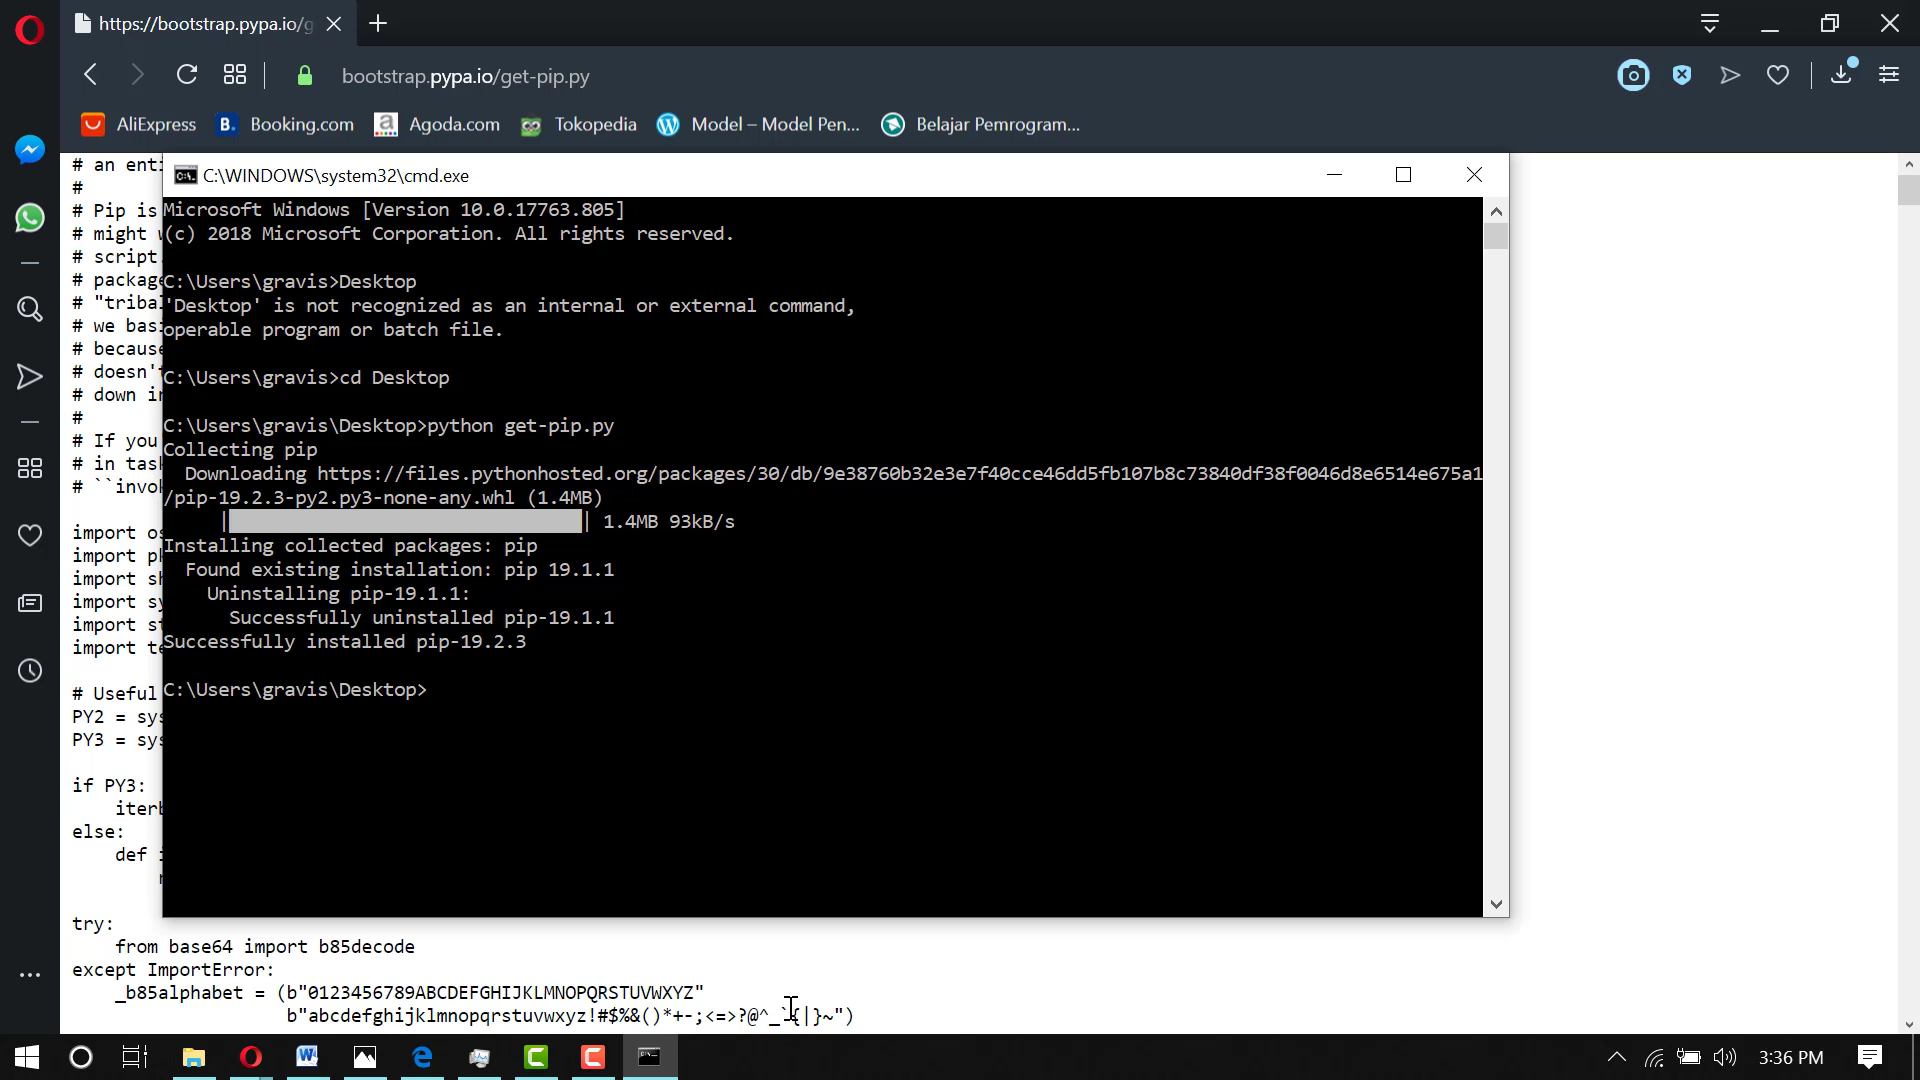
\includegraphics[width=7.5cm]{gambar/pip/Screenshot (79).png} 
\end{itemize}

\chapter{program}
\section{uji coba python lewat interpreter}
\paragraph{}
\begin{itemize}
	\item Buka Command prompt
	\item Tuliskan python lalu enter
	\item tuliskan kode python lalu enter\\
	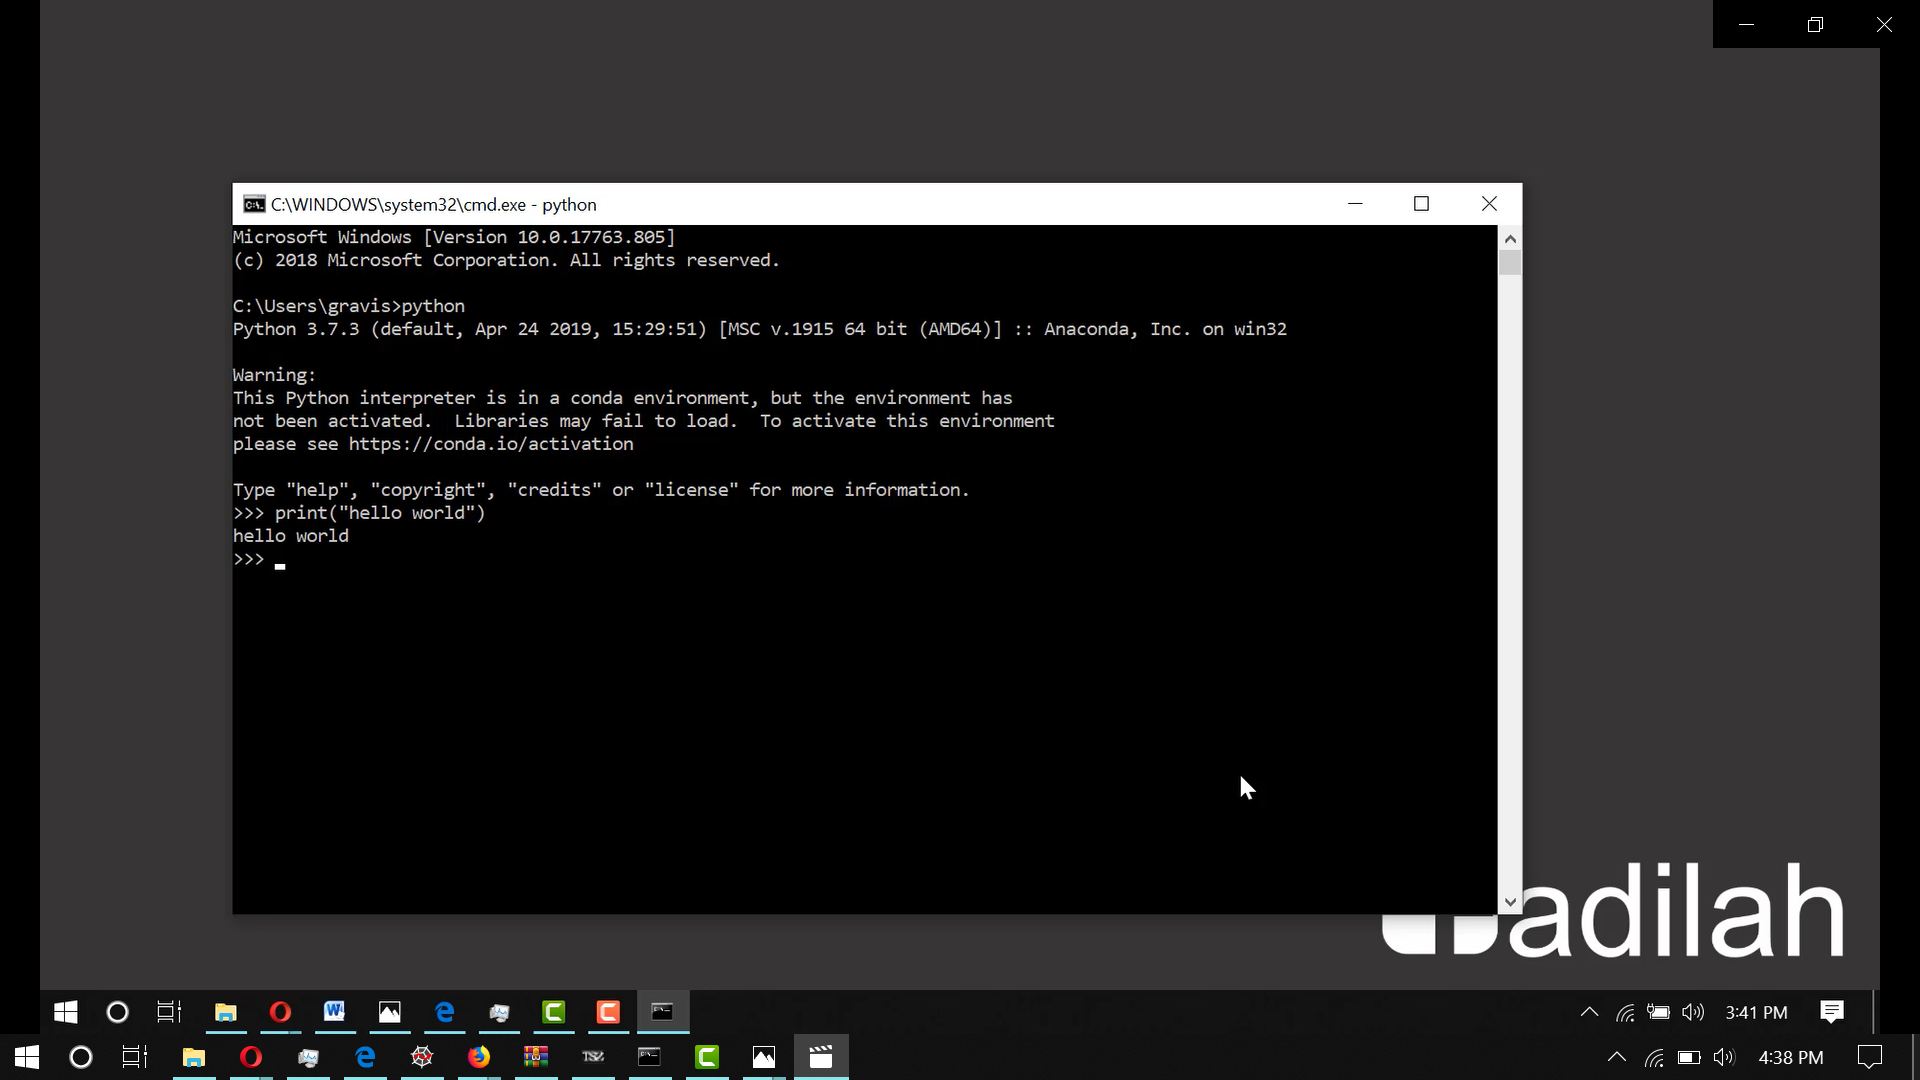
\includegraphics[width=7.5cm]{gambar/entrepreter/Screenshot (80).png} 
	
\end{itemize}

\section{penggunaan spyder}
\subsection{Print hello world}
\paragraph{}
\begin{itemize}
	\item Buka spyder\\
	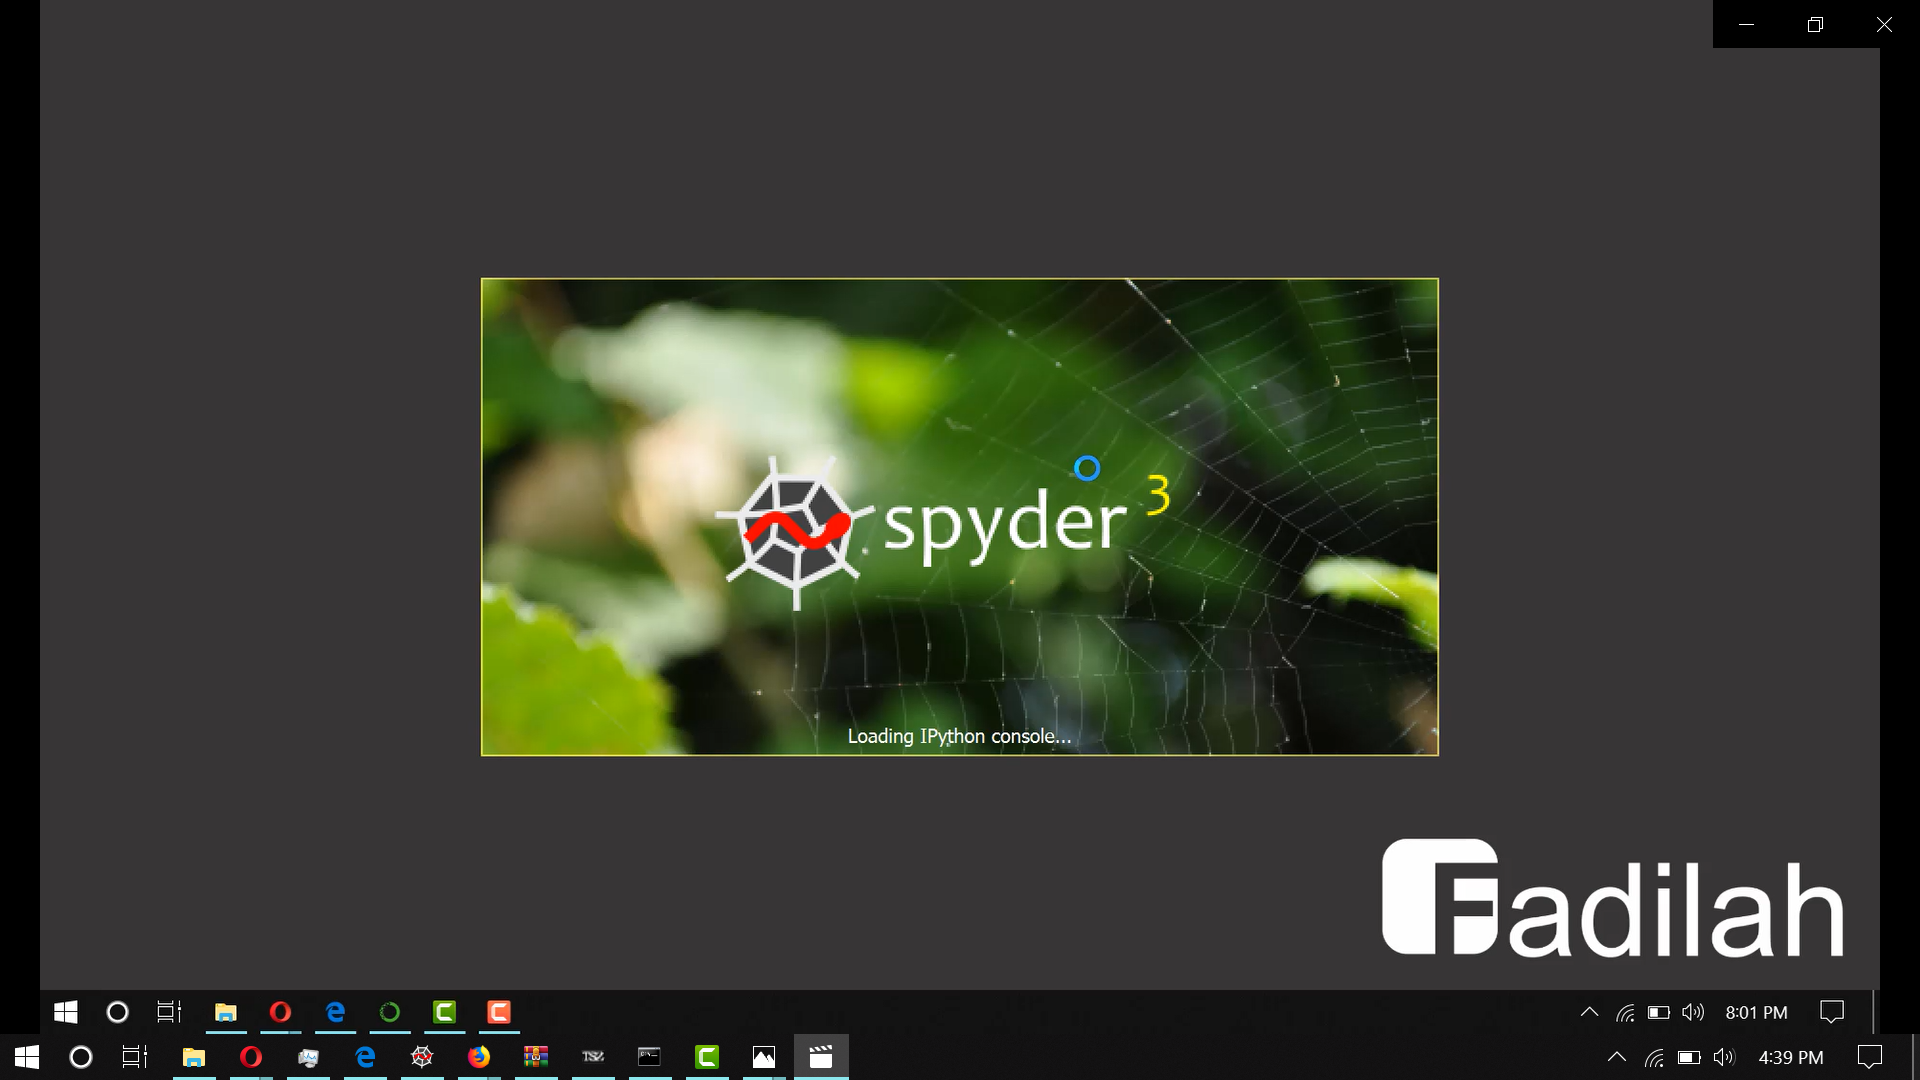
\includegraphics[width=7.5cm]{gambar/spyder/Screenshot (81).png} 
	\item buat file baru CTRL + N\\
	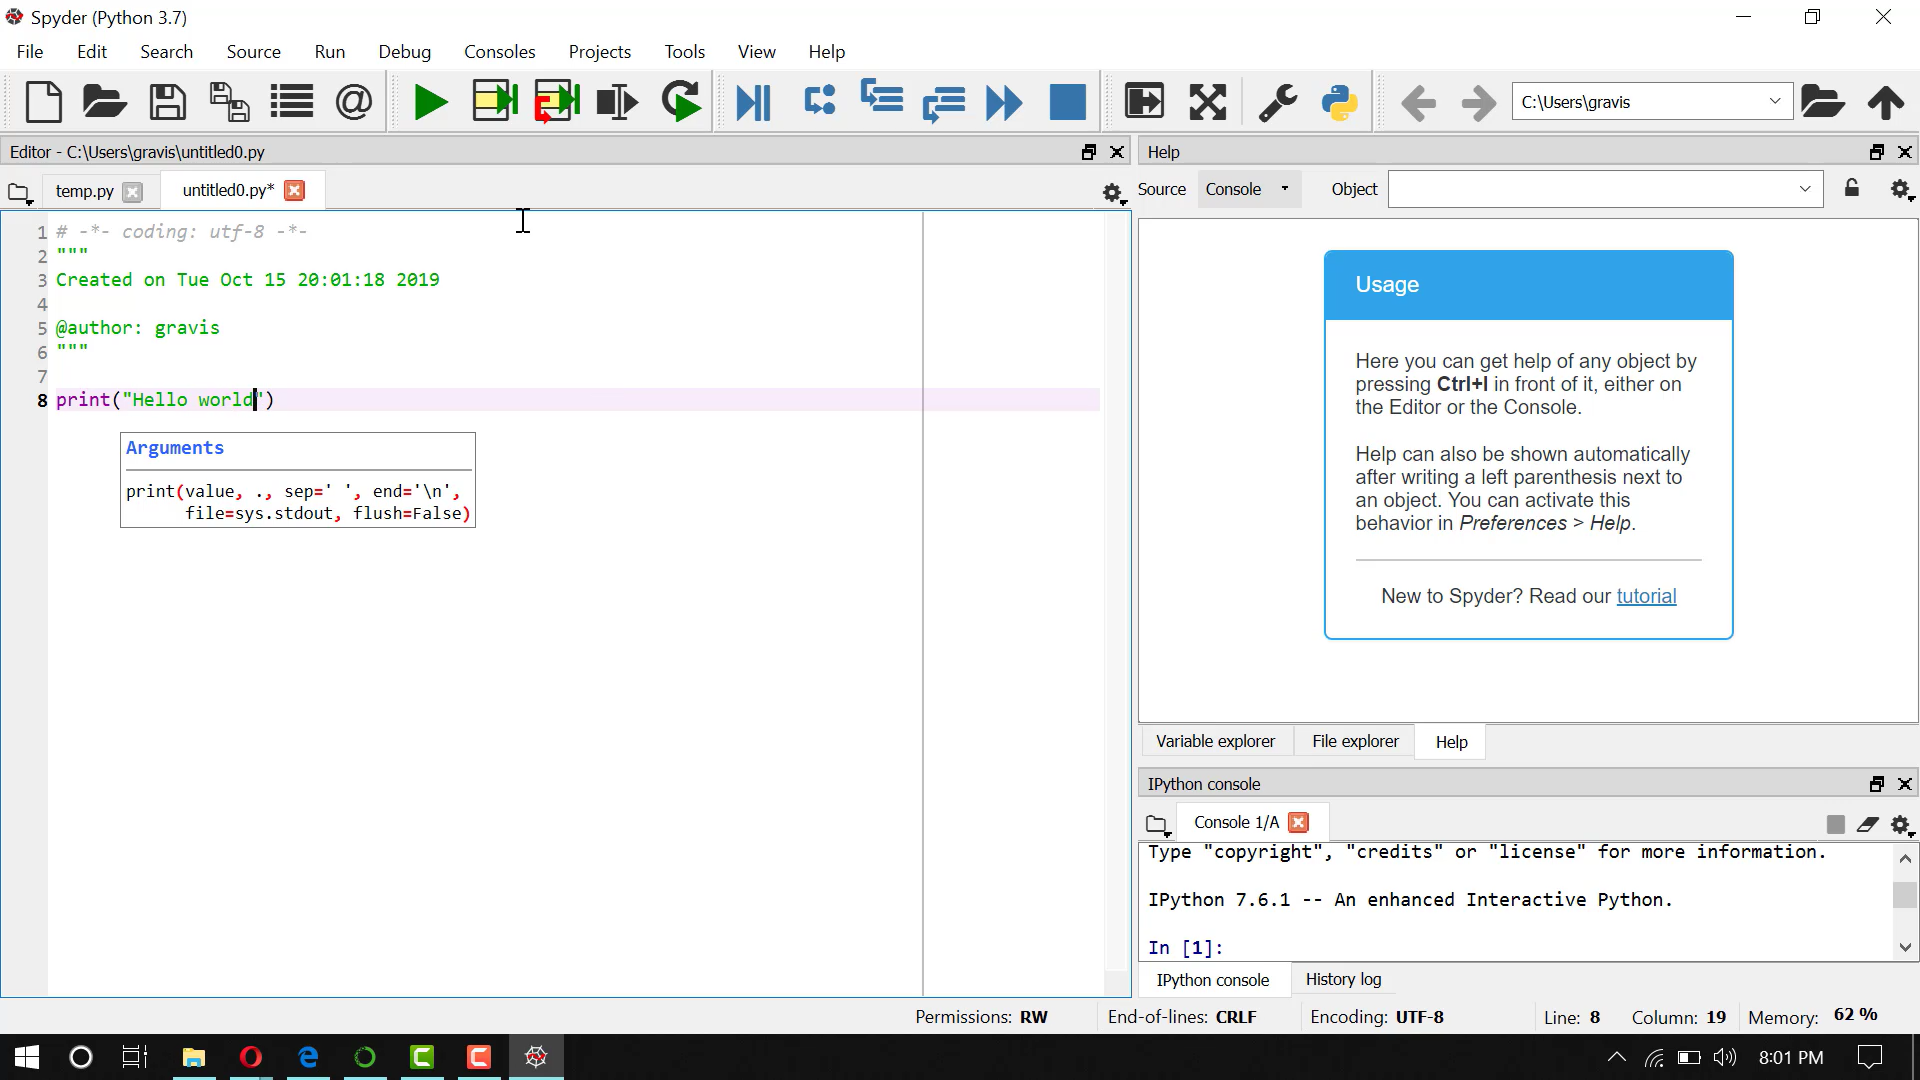
\includegraphics[width=7.5cm]{gambar/spyder/Screenshot (83).png} 
	\item tuliskan syntax "print('hello world')"
	\item klik run script atau tekan F5
	\item tuliskan nama file lalu klik save\\
	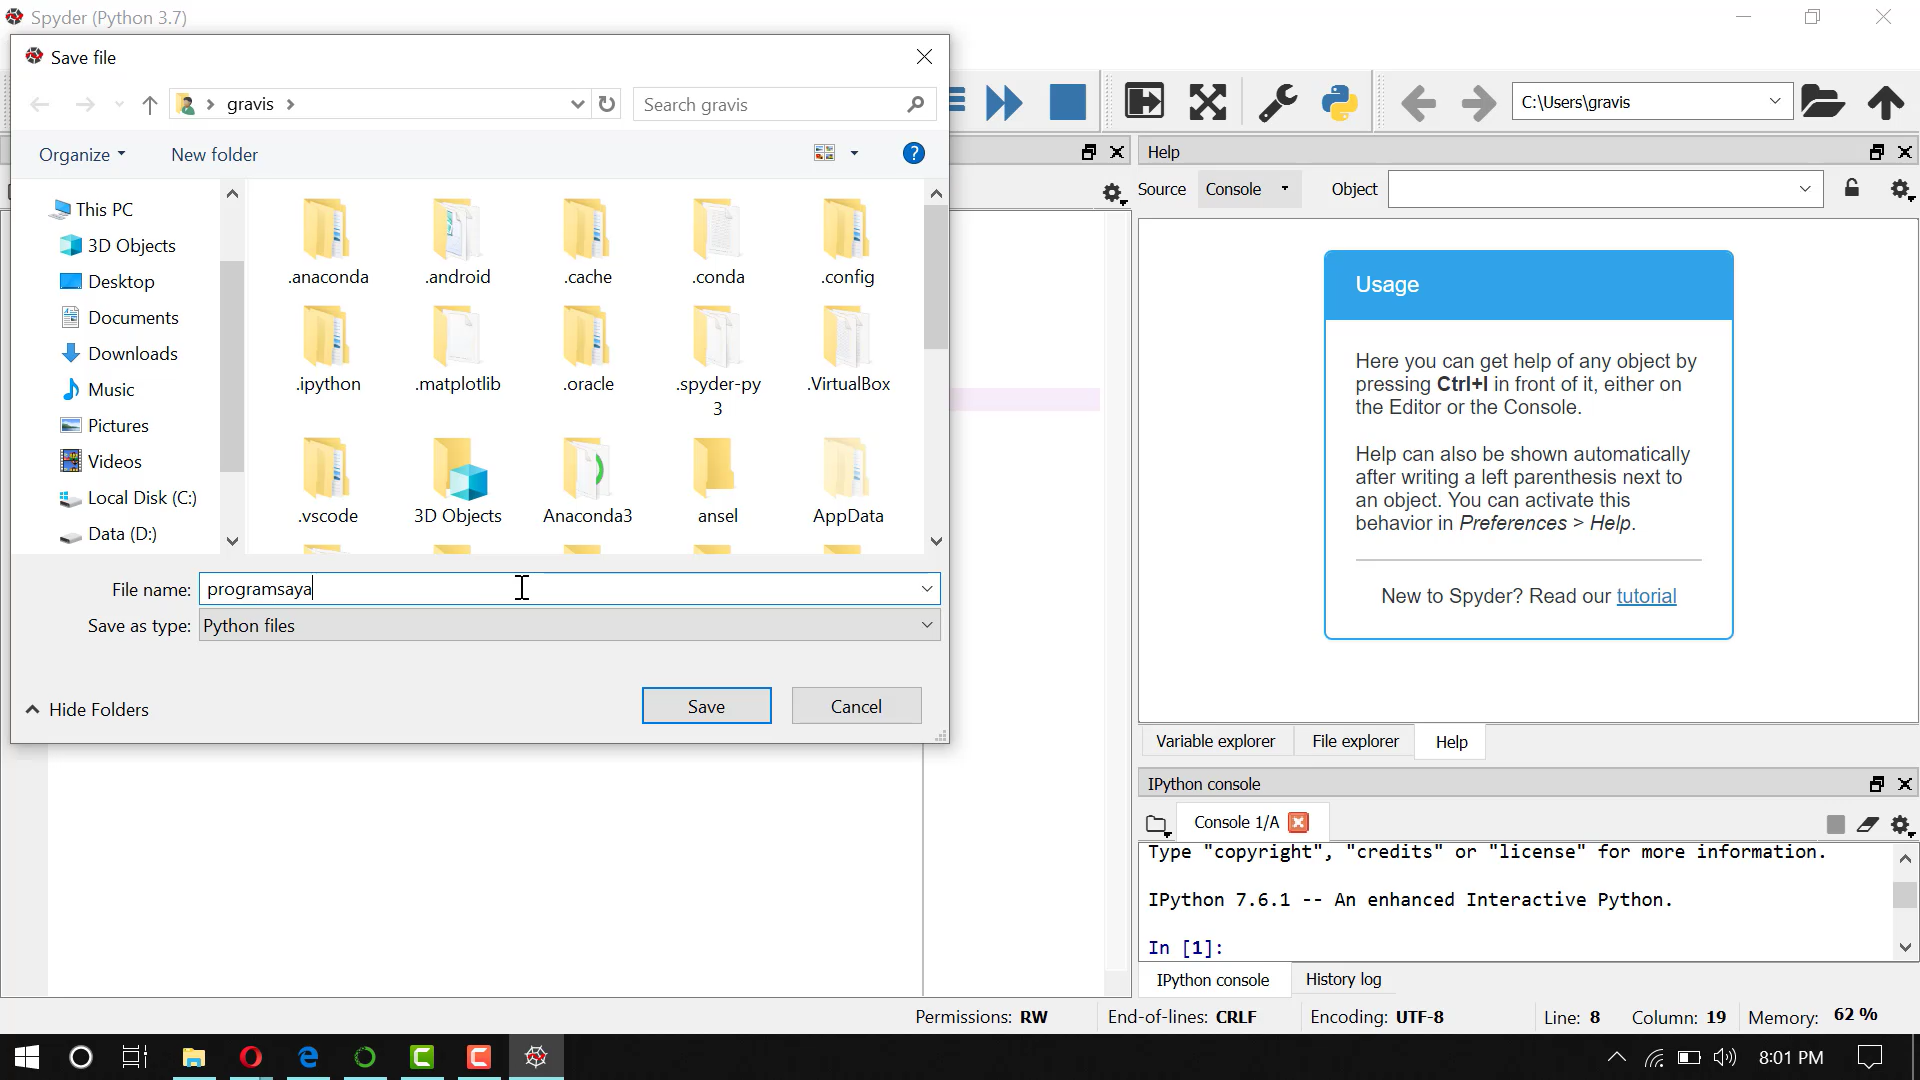
\includegraphics[width=7.5cm]{gambar/spyder/Screenshot (84).png} 
\end{itemize}
\subsection{Penggunaan variable exploler}
\paragraph{}
Variabel exploler digunakan untuk mengecek semua variabel yang mempunyai value, menu bagan variable exploler secara default terletak disebelah kanan\\
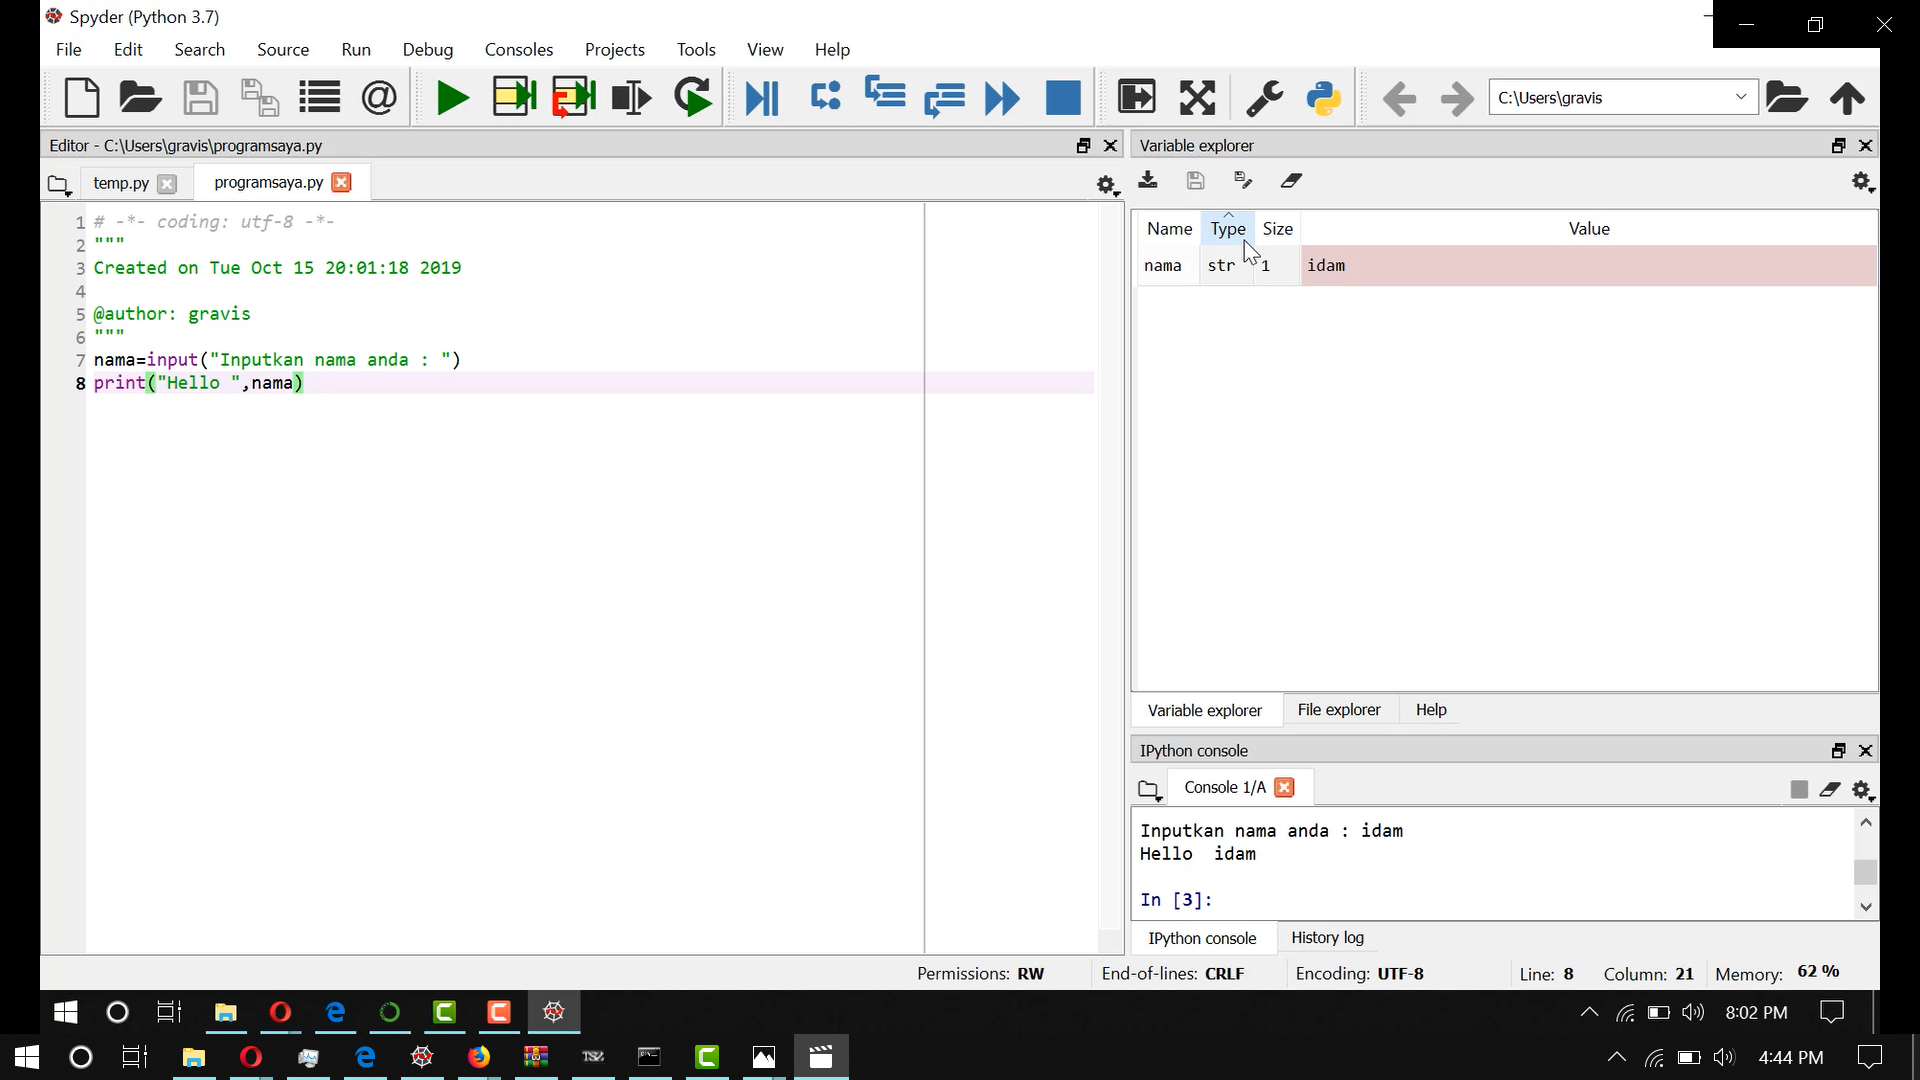
\includegraphics[width=7.5cm]{gambar/spyder/Screenshot (87).png} 
\subsection{Penggunaan library selenium otomatis login untuk website akademik}
\paragraph{}
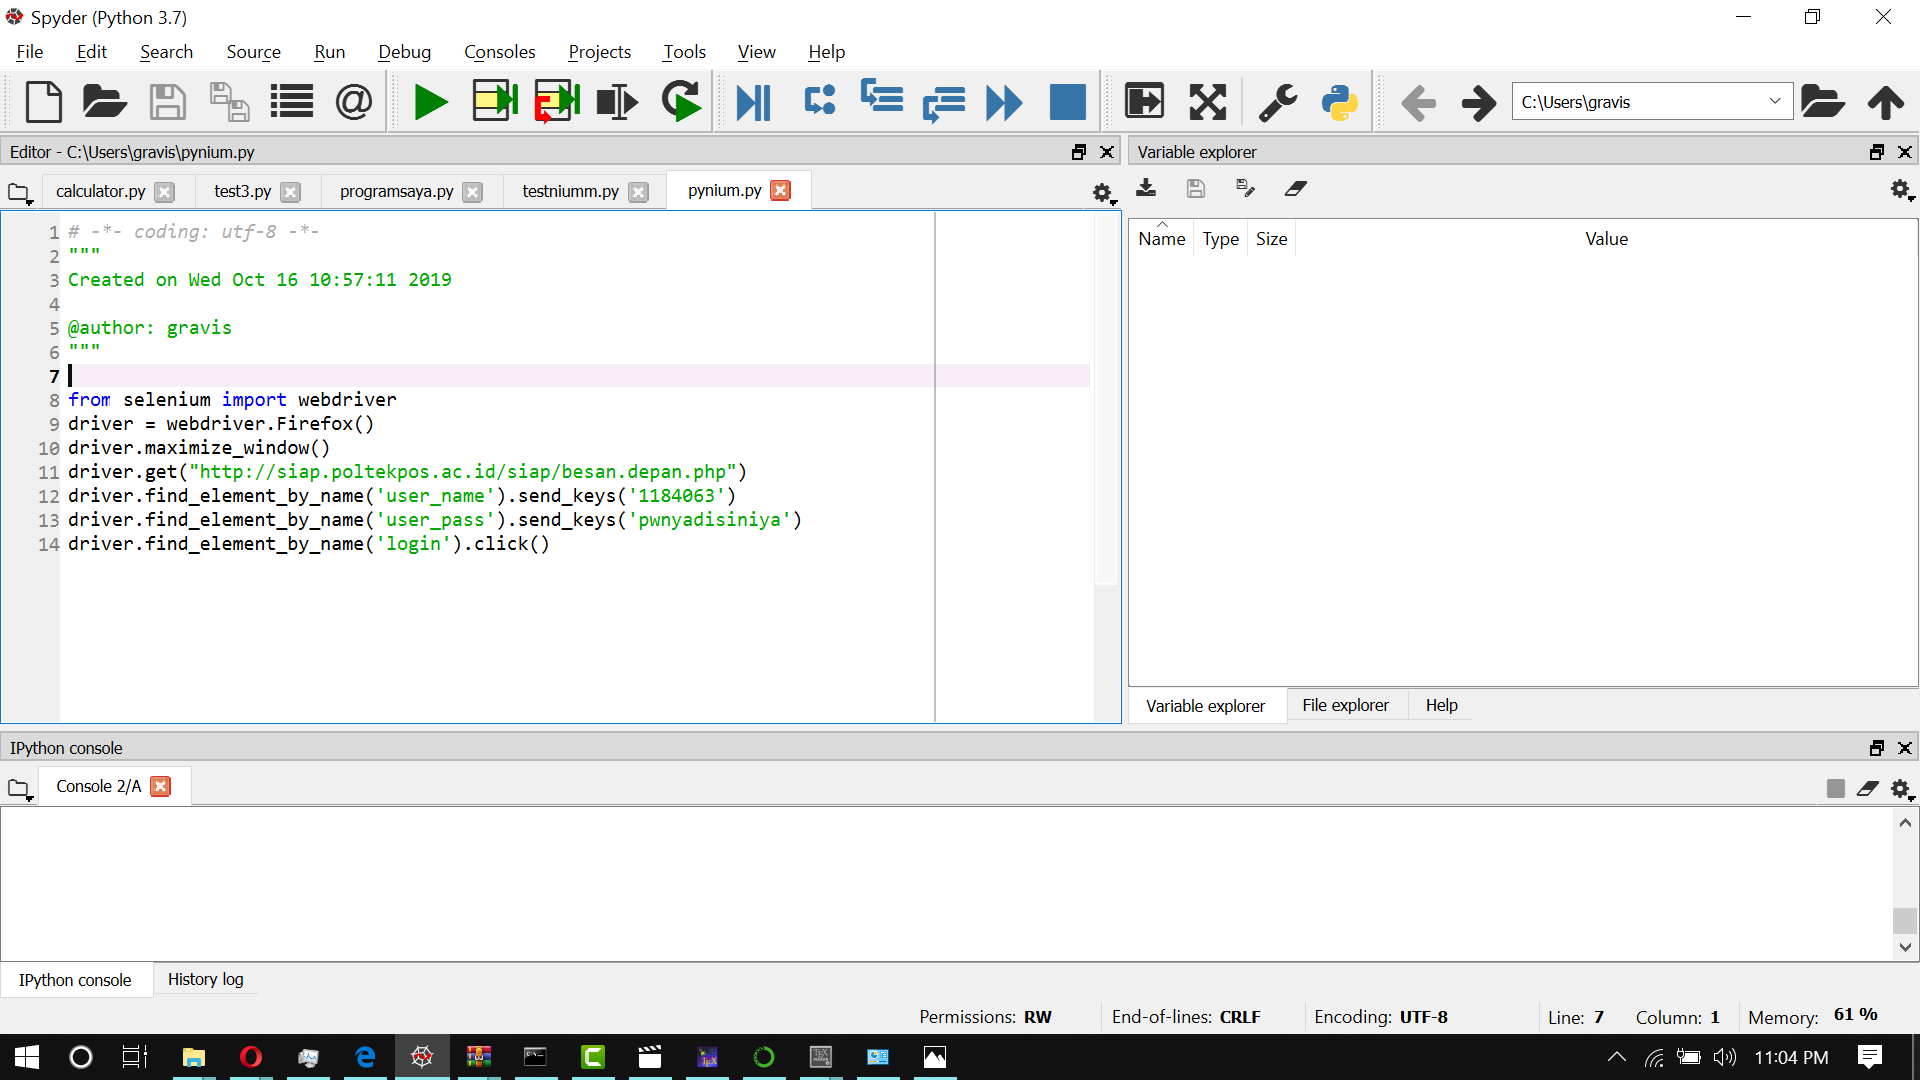
\includegraphics[width=7.5cm]{gambar/spyder/Screenshot (99).png} 
\begin{itemize}
	\item \textbf{from selenium import webdriver}, digunakan untuk import webdriver
	\item \textbf{driver = webdriver.Firefox()}, digunakan untuk memilih webdriver firefox
	\item \textbf{driver.maximize\_window()}, digunakan untuk maximize window browser
	\item \textbf{driver.get("http://siap.poltekpos.ac.id/siap/besan.depan.php")}, digunakan redirect ke website tujuan
	\item \textbf{driver.find\_element\_by\_name('user\_name').send\_keys('1184063')}, digunakan untuk mengisi form username, driver akan mencari element dengan nama user\_name
	\item \textbf{driver.find\_element\_by\_name('user\_pass').send\_keys('pwnyadisiniya')}, digunakan untuk mengisi form password, driver akan mencari element dengan nama pass\_name
	\item \textbf{driver.find\_element\_by\_name('login').click()}, digunakan untuk mengklik tombol login, dengan fungsi click()
\end{itemize}
\chapter{Identasi}
\section{Penjelasan identasi}
\paragraph{}
Indentasi adalah bagian paragraf yang menjorok ke dalam pada baris-baris paragraf, penulisan kode python tidak memakai curly brackets "\{\}" sehingga cara membedakan blok program digunakan identasi.\\
jenis error identasi yaitu \textbf{IndentationError: expected an indented block}.\\
artinya ini berarti fungsi if memerlukan indentasi untuk membedakan blok kode.\\
solusinya yaitu menambahkan indentasi sebelum fungsi print.\\
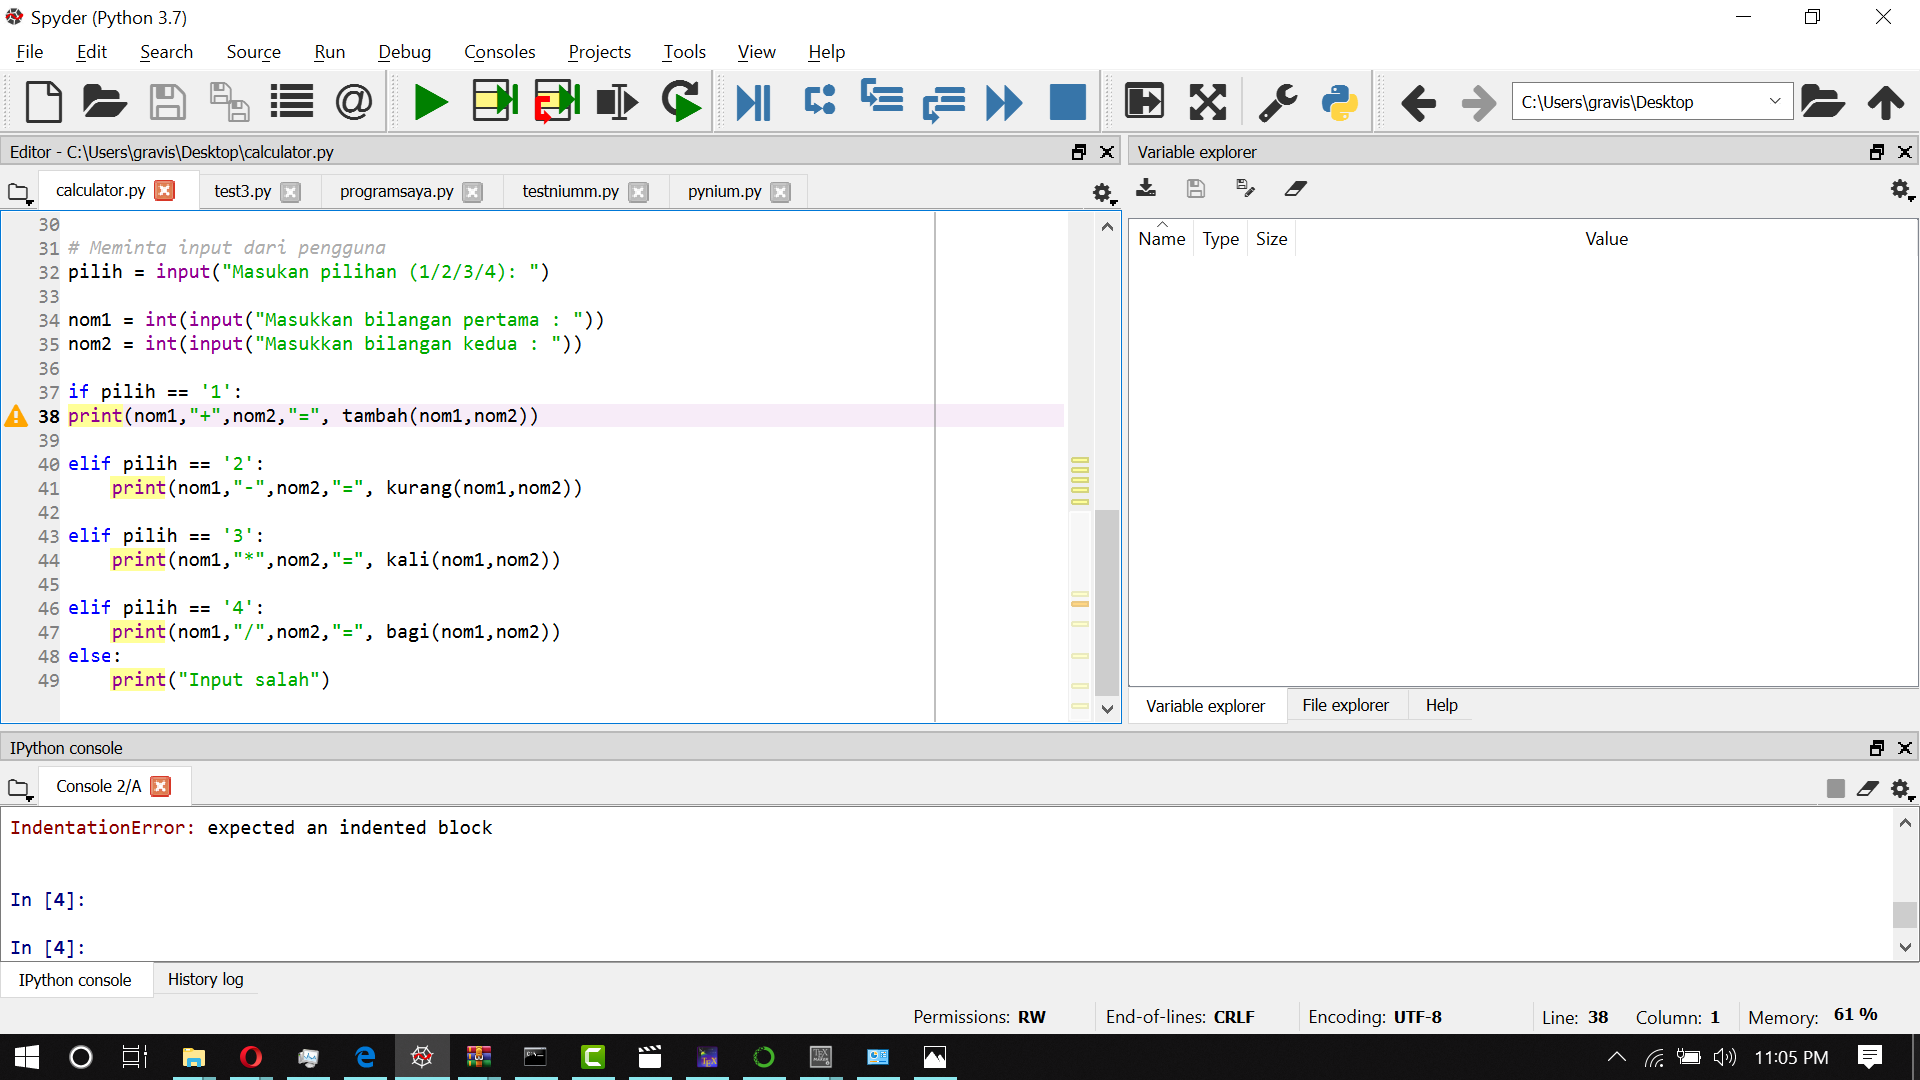
\includegraphics[width=7.5cm]{gambar/spyder/Screenshot (100).png}\\ 
 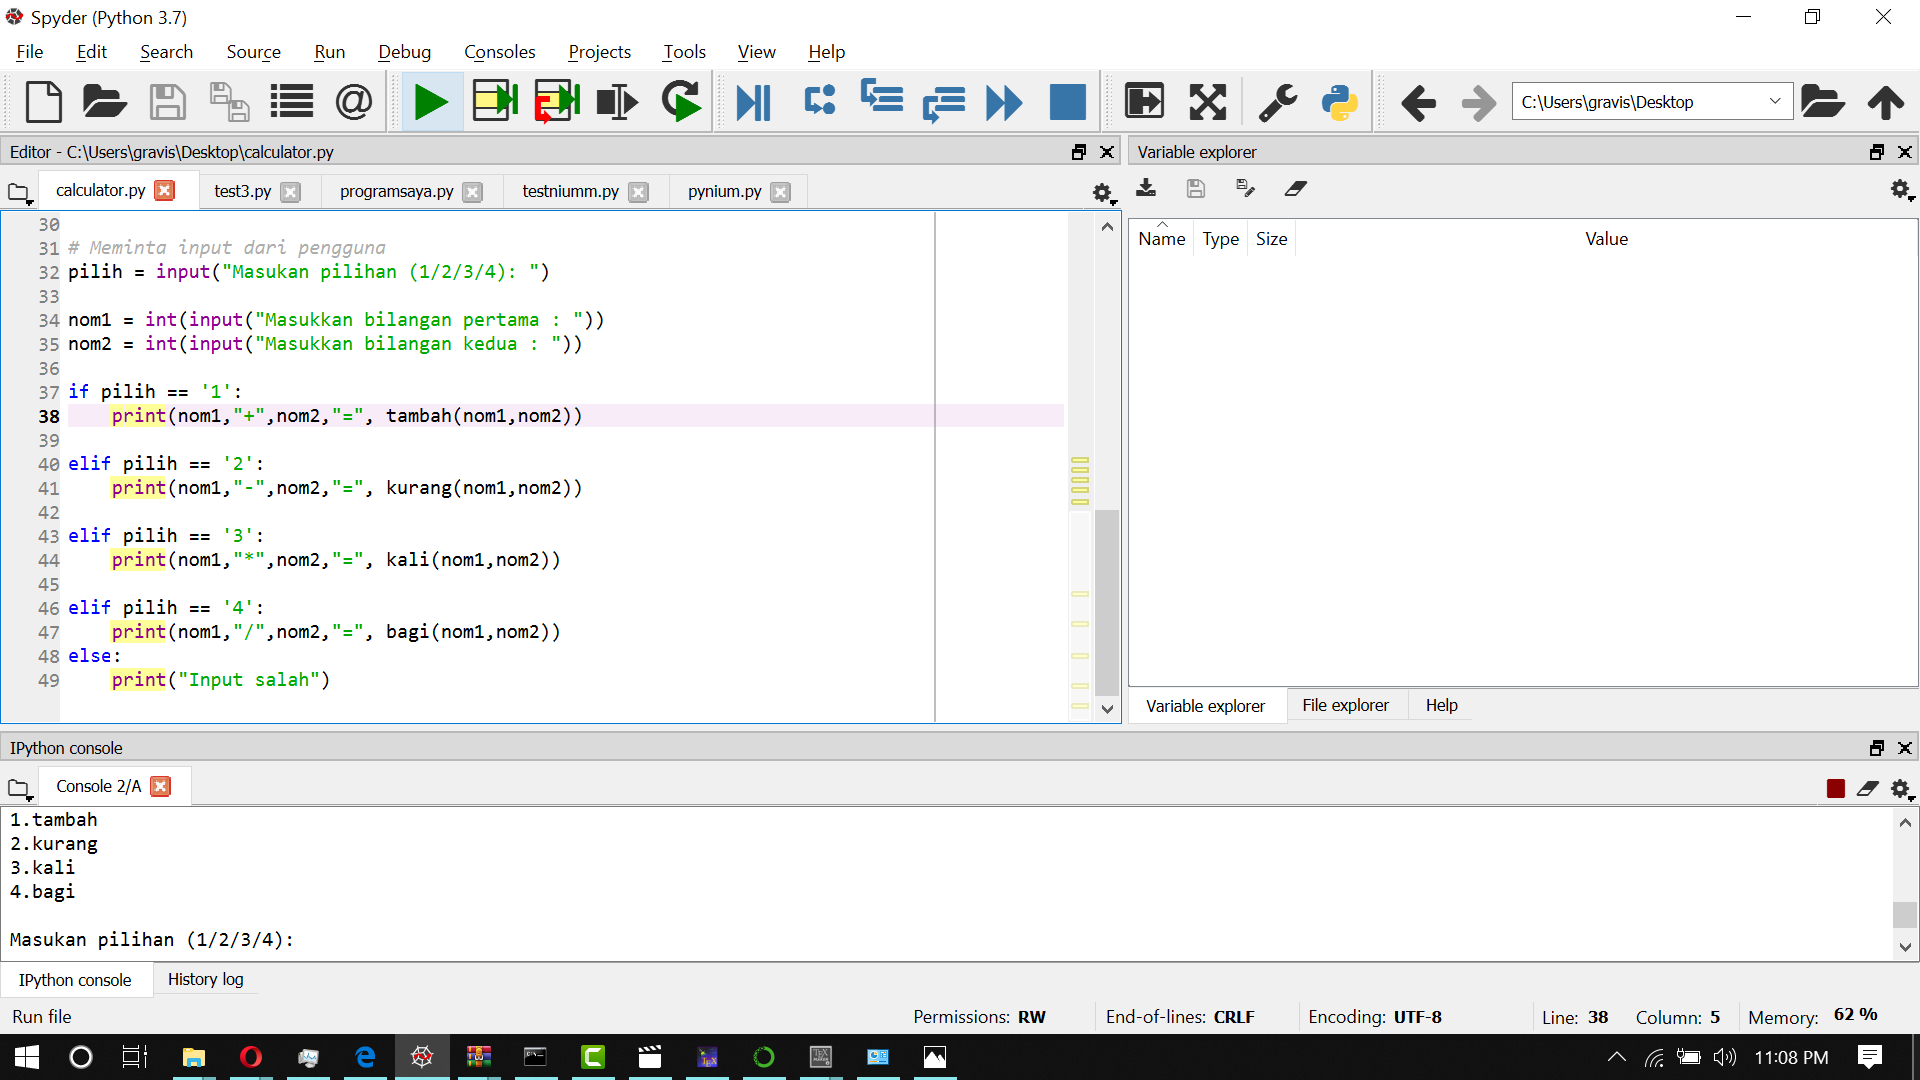
\includegraphics[width=7.5cm]{gambar/spyder/Screenshot (102).png} 
\end{document}